\documentclass{beamer}

\usepackage{epsfig}
\usepackage{multicol}
\usepackage{geometry}
%\usepackage[dvipsnames]{xcolor}
\usepackage{textcomp}
\usepackage{graphicx}
\usepackage{caption}
\usepackage{subcaption}
\usepackage{amsmath}
\usepackage{tcolorbox}
\usetheme{Boadilla}
\usepackage{pict2e}
\usepackage{tikz}
\usepackage{xcolor}
\usepackage[straightvoltages]{circuitikz}


\title[Traitement du signal numérique]{Traitement du signal numérique - HEI4 IMS}
\author[Antony Bazir]{}

\setlength{\unitlength}{1cm}

\begin{document}


\section{Signaux Numériques}
\begin{frame}
\frametitle{Signaux Numériques}
Les transformées de Laplace et Fourier s'appliquent aux signaux continus. Or, on souhaite traiter des \textbf{signaux numériques...}\\

\vspace{1cm}

\only<2->{
\textbf{Comment définit-on des signaux numériques ?}\\
}

\vspace{1cm}

\only<3->{
\textbf{Signal numérique =  codage + échantillonnage}
}

\end{frame} 

\subsubsection{Codage}
\begin{frame}
\frametitle{Codage}
\textbf{Que vous évoque la notion de codage ?}\\
\vspace{1cm}
\only<2->{
\begin{block}{}
Codage : Mode de répresentation discret de l'amplitude caractérisé par des \textbf{quantas} et une \textbf{dynamique}
\end{block}
}

\end{frame}

\begin{frame}
\frametitle{Codage}
Exemple : Deux des manières de coder une fonction rampe de pente 1\\
\vspace{0.3cm}
\only<2->{
\begin{center}
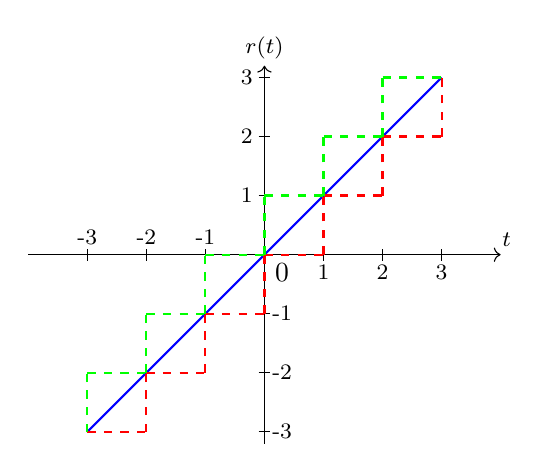
\begin{tikzpicture}
\begin{scope}[scale = 0.75]
\draw[->] (-4,0)-- (4,0);
\draw (0.3,-0.3) node {0};
\draw[->] (0,-3.2)-- (0,3.2);
\draw (4.1,0.25) node {\footnotesize{$t$}};
\draw (0,3.5) node {\footnotesize{$r(t)$}};

\draw (1,-0.1)-- (1,0.1);
\draw (1.0,-0.3) node {\footnotesize{1}};
\draw (2,-0.1)-- (2,0.1);
\draw (2.0,-0.3) node {\footnotesize{2}};
\draw (3,-0.1)-- (3,0.1);
\draw (3.0,-0.3) node {\footnotesize{3}};

\draw (-1,-0.1)-- (-1,0.1);
\draw (-1.0,0.3) node {\footnotesize{-1}};
\draw (-2,-0.1)-- (-2,0.1);
\draw (-2.0,0.3) node {\footnotesize{-2}};
\draw (-3,-0.1)-- (-3,0.1);
\draw (-3.0,0.3) node {\footnotesize{-3}};

\draw (-0.1,1)-- (0.1,1);
\draw (-0.3,1) node {\footnotesize{1}};
\draw (-0.1,2)-- (0.1,2);
\draw (-0.3,2) node {\footnotesize{2}};
\draw (-0.1,3)-- (0.1,3);
\draw (-0.3,3) node {\footnotesize{3}};

\draw (-0.1,-1)-- (0.1,-1);
\draw (0.3,-1) node {\footnotesize{-1}};
\draw (-0.1,-2)-- (0.1,-2);
\draw (0.3,-2) node {\footnotesize{-2}};
\draw (-0.1,-3)-- (0.1,-3);
\draw (0.3,-3) node {\footnotesize{-3}};

%r(t)
\draw[thick,blue] (-3,-3)-- (3,3);

\draw[thick,dashed,red] (-3,-3)-- (-2,-3);
\draw[thick,dashed,red] (-2,-3)-- (-2,-2);
\draw[thick,dashed,red] (-2,-2)-- (-1,-2);
\draw[thick,dashed,red] (-1,-2)-- (-1,-1);
\draw[thick,dashed,red] (-1,-1)-- (-0,-1);
\draw[thick,dashed,red] (-0,-1)-- (-0,-0);
\draw[thick,dashed,red] (-0,-0)-- (1,-0);
\draw[thick,dashed,red] (1,0)-- (1,1);
\draw[thick,dashed,red] (1,1)-- (2,1);
\draw[thick,dashed,red] (2,1)-- (2,2);
\draw[thick,dashed,red] (2,2)-- (3,2);
\draw[thick,dashed,red] (3,2)-- (3,3);

\draw[thick,dashed,green] (-3,-2)-- (-2,-2);
\draw[thick,dashed,green] (-3,-3)-- (-3,-2);
\draw[thick,dashed,green] (-2,-1)-- (-1,-1);
\draw[thick,dashed,green] (-2,-2)-- (-2,-1);
\draw[thick,dashed,green] (-1,-0)-- (-0,-0);
\draw[thick,dashed,green] (-1,-1)-- (-1,0);
\draw[thick,dashed,green] (-0,1)-- (1,1);
\draw[thick,dashed,green] (0,0)-- (0,1);
\draw[thick,dashed,green] (1,2)-- (2,2);
\draw[thick,dashed,green] (1,1)-- (1,2);
\draw[thick,dashed,green] (2,3)-- (3,3);
\draw[thick,dashed,green] (2,2)-- (2,3);
\end{scope}
\end{tikzpicture}
\end{center}
}
\vspace{0.3cm}
\only<3->{
Ici le quanta vaut 1 unité et la gamme dynamique est de 6 quanta
}

\end{frame}

\begin{frame}
\frametitle{Codage} 
\textbf{Exercice: Supposons qu'on code un signal d'une amplitude de crête de 5 volts sur 4 bits}\\
\vspace{1cm}
\begin{itemize}
\item<2-> De combien de valeurs dispose-t-on pour coder la gamme dynamique ?  \only<4->{\textbf{16 valeurs: [0,15]}}
\vspace{0.2cm}
\item<3-> Quelle est la valeur d'un quanta/échelon de quantification ? \only<5->{$q$ = \textbf{0.625 V}} 
\end{itemize}

\end{frame} 


\begin{frame}
\frametitle{Codage: Aspects pratiques}
Le codage est... \textbf{partout}\\
\vspace{0.2cm}
\begin{itemize}
\item Résolution de \textbf{tous} les appareils de mesures numériques
\item Représentation et reproduction de valeurs sur les ordinateurs
\item Tout le traitement du signal numérique
\end{itemize}
\end{frame}

\begin{frame}
\frametitle{Codage: Aspects pratiques}
Le codage est... \textbf{partout}\\
\vspace{0.2cm}
\includegraphics[scale=0.45]{8_12_bits.png}\\
\center{\footnotesize{\textit{Illustration de la résolution à 8 et 12 bits (LeCroy)}}}
\vspace{0.2cm}
\begin{itemize}
\item Compromis résolution/stockage
\vspace{0.1cm}
\item Potentielle difficulté à trouver le signal d'intérêt
\vspace{0.1cm}
\item On ne connaît pas forcément bien le signal recherché
\end{itemize}
\end{frame}


\begin{frame}
\frametitle{Codage: Aspects pratiques}
Le codage est... \textbf{partout}\\
\begin{columns}
\column{60mm}
\includegraphics[scale=0.25]{err_quantif.png}\\
\center{\footnotesize{\textit{Illustration de l'erreur de quantification (Bellanger)}}}
\column{60mm}
\begin{itemize}
\item Plusieurs choix possibles pour le codage
\vspace{0.1cm}
\item Choix dépendant du type de signal
\vspace{0.1cm}
\item On peut aussi adapter la dynamique pour réduire l'erreur dans certains cas
\end{itemize}
\end{columns}
\end{frame}


\subsubsection{Echantillonnage} 
\begin{frame} 
\frametitle{\'Echantillonnage} 

\textbf{Question : En quoi consiste pour vous l'opération d'échantillonnage ?}\\
\vspace{0.5cm}
\only<2->{
\begin{block}{}
"L’échantillonnage consiste à représenter un signal fonction du temps $s(t)$ par ses
valeurs $s(nT_e)$ à des instants multiples entiers d’une durée $T_e$, appelée période d’échantillonnage."\footnotesize {M. Bellanger}
\end{block}
}
\end{frame}

\begin{frame}
\frametitle{\'Echantillonnage : Peigne de Dirac}

L'opération d'échantillonnage s'appuie sur la distribution appelée "peigne de Dirac"\\

\vspace{0.7cm} 

 \[ u_{T_e}(t) = \sum_{n = -\infty}^{\infty} \delta(t-nT_e) \]\\
 
\vspace{0.7cm}
On a alors\\

\vspace{0.3cm}

 \[\boxed{s(nT_e) = s(t) \cdot u_{T_e}(t)}\]
\end{frame}

\begin{frame}
\frametitle{\'Echantillonnage: exemple}
\begin{columns}
\column{60mm}
\begin{center}
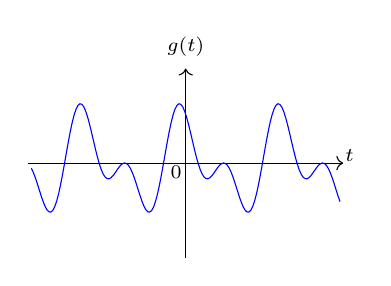
\begin{tikzpicture}
\begin{scope}[scale=0.4]
	\draw[->] (-5,0)-- (5,0);
\draw (-0.3,-0.3) node {\scriptsize{0}};
\draw[->] (0,-3)-- (0,3);
\draw (5.2,0.25) node {\scriptsize $t$};
\draw (0,3.7) node {\scriptsize $g(t)$};
%\draw (4.5,-0.3) node {1};

\draw[domain=-4.9:4.9,color=blue,samples=160] plot (\x,{2*(0.55*cos(2*\x r)+ 0.45*cos(2*2*(\x+3.14/12) r))});
\end{scope}
	\end{tikzpicture}
\end{center}
\column{60mm}
\begin{center}
\begin{tikzpicture}
\begin{scope}[scale=0.4]
	\draw[->] (-5,0)-- (5,0);
%\draw (-0.3,-0.3) node {0};
\draw[->] (0,-3)-- (0,3);
\draw (5.3,0.25) node {\scriptsize $t$};
\draw (0,3.7) node {\scriptsize $u_{T_e}(t)$};
%\draw (4.5,-0.3) node {1};

\draw[thick,blue] (-4,-0)-- (-4,1);
\draw[thick,blue] (-3.5,-0)-- (-3.5,1);
\draw[thick,blue] (-3,-0)-- (-3,1);
\draw[thick,blue] (-2.5,-0)-- (-2.5,1);
\draw[thick,blue] (-2,-0)-- (-2,1);
\draw[thick,blue] (-1.5,-0)-- (-1.5,1);
\draw[thick,blue] (-1,-0)-- (-1,1);
\draw[thick,blue] (-0.5,-0)-- (-0.5,1);
\draw[thick,blue] (0,-0)-- (0,1);
\draw[thick,blue] (0.5,-0)-- (0.5,1);
\draw[thick,blue] (1,-0)-- (1,1);
\draw[thick,blue] (1.5,-0)-- (1.5,1);
\draw[thick,blue] (2,-0)-- (2,1);
\draw[thick,blue] (2.5,-0)-- (2.5,1);
\draw[thick,blue] (3,-0)-- (3,1);
\draw[thick,blue] (3.5,-0)-- (3.5,1);
\draw[thick,blue] (4,-0)-- (4,1);
\end{scope}
	\end{tikzpicture}
\end{center}

\end{columns}
Si on prend le produit des deux fonctions, on obtient: 
\begin{center}
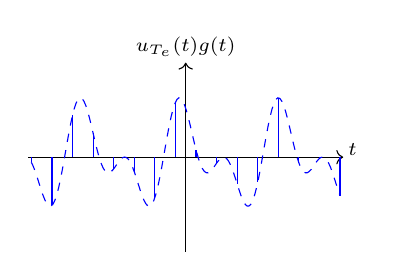
\begin{tikzpicture}
\begin{scope}[scale=0.4]
	\draw[->] (-5,0)-- (5,0);
%\draw (-0.3,-0.3) node {0};
\draw[->] (0,-3)-- (0,3);
\draw (5.3,0.25) node {\scriptsize $t$};
\draw (0,3.5) node {\scriptsize $u_{T_{e}}(t)g(t)$};
%\draw (4.5,-0.3) node {1};

\draw[dashed,domain=-4.9:4.9,color=blue,samples=160] plot (\x,{2*(0.55*cos(2*\x r)+ 0.45*cos(2*2*(\x+3.14/12) r))});

\draw[domain=-4.9:4.9,color=blue,samples=16] plot[ycomb] (\x,{2*(0.55*cos(2*\x r)+ 0.45*cos(2*2*(\x+3.14/12) r))});
%\draw[ domain=0.1:4.9,color=blue,samples=24] plot[ycomb] (\x,{80*abs(sin(5*3.14*\x r -5*3.14*2.5r )/(5*3.14*\x r-5*3.14*2.5 r))});
%\draw[thick,blue] (-4,-0)-- (-4,-0.9);
%\draw[thick,blue] (-3,-0)-- (-3,1);
%\draw[thick,blue] (-2,-0)-- (-2,0);
%\draw[thick,blue] (-1,-0)-- (-1,-1.25);
%\draw[thick,blue] (0,-0)-- (0,1.3);
%\draw[thick,blue] (1,-0)-- (1,-0.15);
%\draw[thick,blue] (2,-0)-- (2,-1.5);
%\draw[thick,blue] (3,-0)-- (3,1.8);
%\draw[thick,blue] (4,-0)-- (4,-0.35);
\end{scope}
	\end{tikzpicture}
\end{center}
\end{frame}
 
 
\begin{frame}
\frametitle{\'Echantillonnage: exemple}
On souhaite échantillonner le signal : $$ g(t) = 0.55\cos(2 t) + 0.45 \cos(4 t + \frac{\pi}{3}) $$ 
\only<2->{
\begin{center}
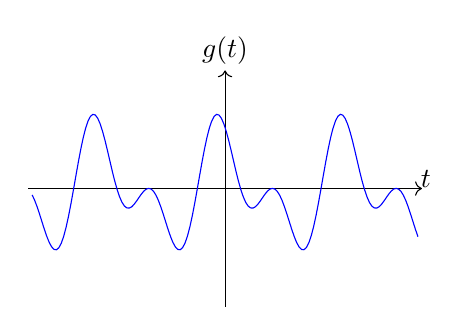
\begin{tikzpicture}
\begin{scope}[scale=0.5]
	\draw[->] (-5,0)-- (5,0);
%\draw (-0.3,-0.3) node {0};
\draw[->] (0,-3)-- (0,3);
\draw (5.1,0.25) node {$t$};
\draw (0,3.5) node {$g(t)$};
%\draw (4.5,-0.3) node {1};

\draw[domain=-4.9:4.9,color=blue,samples=160] plot (\x,{2*(0.55*cos(2*\x r)+ 0.45*cos(2*2*(\x+3.14/12) r))});
\end{scope}
	\end{tikzpicture}
\end{center}
}

\end{frame}

\begin{frame}
\frametitle{\'Echantillonnage: exemple}
On souhaite échantillonner le signal : $$ g(t) = 0.55\cos(2 t) + 0.45 \cos(4 t + \frac{\pi}{3}) $$ 
\only<2->{
\begin{center}
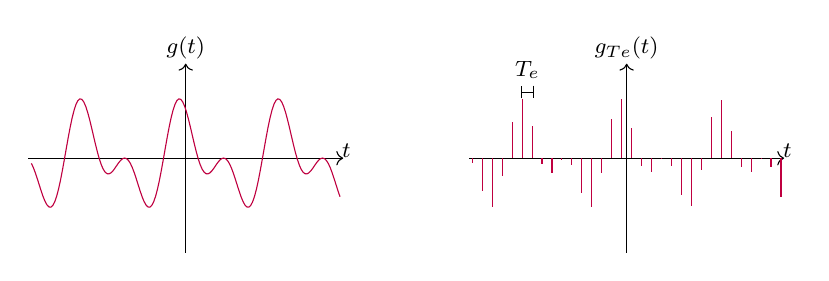
\begin{tikzpicture}
\begin{scope}[scale=0.4]
	\draw[->] (-5,0)-- (5,0);
%\draw (-0.3,-0.3) node {0};
\draw[->] (0,-3)-- (0,3);
\draw (5.1,0.25) node {\footnotesize{$t$}};
\draw (0,3.5) node {\footnotesize{$g(t)$}};
%\draw (4.5,-0.3) node {1};

\draw[domain=-4.9:4.9,color=purple,samples=160] plot (\x,{2*(0.55*cos(2*\x r)+ 0.45*cos(2*2*(\x+3.14/12) r))});
\end{scope}

\begin{scope}[scale=0.4,xshift=14cm]
	\draw[->] (-5,0)-- (5,0);
%\draw (-0.3,-0.3) node {0};
\draw[->] (0,-3)-- (0,3);
\draw (5.1,0.25) node {\footnotesize{$t$}};
\draw (0,3.5) node {\footnotesize{$g_{Te}(t)$}};
%\draw (4.5,-0.3) node {1};
\draw[|-|] (-2.95,2.1)--(-3.35,2.1);
\draw (-3.15,2.8) node {\footnotesize{$T_e$}};

\draw[domain=-4.9:4.9,color=purple,samples=32] plot[ycomb] (\x,{2*(0.55*cos(2*\x r)+ 0.45*cos(2*2*(\x+3.14/12) r))});
\end{scope}
	\end{tikzpicture}
\end{center}
}

\end{frame}

\begin{frame}
\frametitle{\'Echantillonnage: exemple}
On souhaite échantillonner le signal : $ g(t) = 0.55\cos(2 t) + 0.45 \cos(4 t + \frac{\pi}{3}) $\\
\vspace{0.3cm}
On échantillonne à 3 périodes : $T_1$ $<$ $T_2$ $<$ $T_3$

\begin{center}
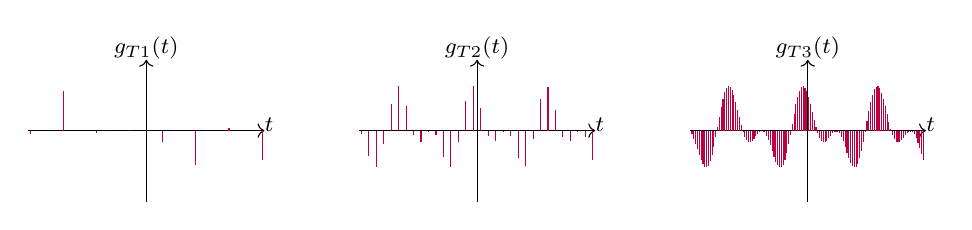
\begin{tikzpicture}
\begin{scope}[scale=0.3,xshift=0cm]
	\draw[->] (-5,0)-- (5,0);
%\draw (-0.3,-0.3) node {0};
\draw[->] (0,-3)-- (0,3);
\draw (5.2,0.25) node {\footnotesize{$t$}};
\draw (0,3.5) node {\footnotesize{$g_{T1}(t)$}};
%\draw (4.5,-0.3) node {1};
%\draw[|-|] (-2.95,2.1)--(-3.35,2.1);
%\draw (-3.15,2.8) node {\footnotesize{$T_1$}};

\draw[domain=-4.9:4.9,color=purple,samples=8] plot[ycomb] (\x,{2*(0.55*cos(2*\x r)+ 0.45*cos(2*2*(\x+3.14/12) r))});
\end{scope}

\begin{scope}[scale=0.3,xshift=14cm]
	\draw[->] (-5,0)-- (5,0);
%\draw (-0.3,-0.3) node {0};
\draw[->] (0,-3)-- (0,3);
\draw (5.2,0.25) node {\footnotesize{$t$}};
\draw (0,3.5) node {\footnotesize{$g_{T2}(t)$}};
%\draw (4.5,-0.3) node {1};
%\draw[|-|] (-2.95,2.1)--(-3.35,2.1);
%\draw (-3.15,2.8) node {\footnotesize{$T_2$}};

\draw[domain=-4.9:4.9,color=purple,samples=32] plot[ycomb] (\x,{2*(0.55*cos(2*\x r)+ 0.45*cos(2*2*(\x+3.14/12) r))});
\end{scope}

\begin{scope}[scale=0.3,xshift=28cm]
	\draw[->] (-5,0)-- (5,0);
%\draw (-0.3,-0.3) node {0};
\draw[->] (0,-3)-- (0,3);
\draw (5.2,0.25) node {\footnotesize{$t$}};
\draw (0,3.5) node {\footnotesize{$g_{T3}(t)$}};
%\draw (4.5,-0.3) node {1};
%\draw[|-|] (-2.95,2.1)--(-3.35,2.1);
%\draw (-3.15,2.8) node {\footnotesize{$T_3$}};

\draw[domain=-4.9:4.9,color=purple,samples=128] plot[ycomb] (\x,{2*(0.55*cos(2*\x r)+ 0.45*cos(2*2*(\x+3.14/12) r))});
\end{scope}
	\end{tikzpicture}
\end{center}

On ne reconnaît plus le signal car $T_1$ est trop élevée...

\begin{block}{}
Comment choisir $T_e$ pour éviter la perte d'information ?
\end{block}

\end{frame}

\begin{frame} 
\frametitle{\'Echantillonnage: exemple}
\begin{block}{Critère de Shannon}
Pour échantillonner un signal sans perte d'information, il faut que la fréquence d'échantillonnage soit deux fois supérieure à la fréquence maximale présente dans le signal
\end{block}
\only<2->{
\vspace{0.4cm}
$g(t) = 0.55\cos(2 t) + 0.45 \cos(4 t + \frac{\pi}{3}) \rightarrow \nu_e = $ ?\\
}


\end{frame}

\begin{frame}
\frametitle{\'Echantillonnage: exemple}
On souhaite échantillonner le signal : $$g(t) = 0.55{\color{blue}\cos(2 t)} + 0.45 \cos(4 t + \frac{\pi}{3}) $$
\begin{columns}[T]
\column{60 mm}
\begin{center}
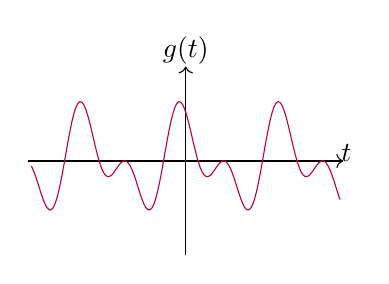
\begin{tikzpicture}
\begin{scope}[scale=0.4,yshift=-1cm]
	\draw[->] (-5,0)-- (5,0);
%\draw (-0.3,-0.3) node {0};
\draw[->] (0,-3)-- (0,3);
\draw (5.1,0.25) node {$t$};
\draw (0,3.5) node {$g(t)$};
%\draw (4.5,-0.3) node {1};

\draw[domain=-4.9:4.9,color=purple,samples=160] plot (\x,{2*(0.55*cos(2*\x r)+ 0.45*cos(2*2*(\x+3.14/12) r))});
\end{scope}
	\end{tikzpicture}
\end{center}

\column{60 mm}

Quelles sont les composantes en fréquence de ce signal ?\\
\vspace{0.3cm}
Méthode directe :\\
\vspace{0.3cm}
\only<2->{
$\cos(2\pi\nu t) \rightarrow \nu$\\
\vspace{0.3cm}
\only<3->{
$ \cos(2\pi\nu t) = \cos(2t) \rightarrow  2\pi\nu = 2 $ \\
\vspace{0.3cm}
\only<4->{
{\color{blue}$\rightarrow \nu = 1/\pi$}
}
}
}

\end{columns}
\end{frame}


\begin{frame}
\frametitle{\'Echantillonnage: exemple}
On souhaite échantillonner le signal : $$g(t) = 0.55\cos(2 t) + 0.45 {\color{red}\cos(4 t + \frac{\pi}{3})} $$
\begin{columns}[T]
\column{60 mm}
\begin{center}
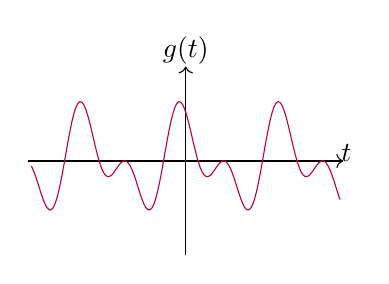
\begin{tikzpicture}
\begin{scope}[scale=0.4,yshift=-1cm]
	\draw[->] (-5,0)-- (5,0);
%\draw (-0.3,-0.3) node {0};
\draw[->] (0,-3)-- (0,3);
\draw (5.1,0.25) node {$t$};
\draw (0,3.5) node {$g(t)$};
%\draw (4.5,-0.3) node {1};

\draw[domain=-4.9:4.9,color=purple,samples=160] plot (\x,{2*(0.55*cos(2*\x r)+ 0.45*cos(2*2*(\x+3.14/12) r))});
\end{scope}
	\end{tikzpicture}
\end{center}

\column{60 mm}

Quelles sont les composantes en fréquence de ce signal ?\\
\vspace{0.3cm}
Méthode directe :\\
\vspace{0.3cm}
\only<2->{
$\cos(2\pi\nu t) \rightarrow \nu$\\
\vspace{0.3cm}
\only<3->{
$ \cos(2\pi\nu t) = \cos(4t) \rightarrow  2\pi\nu = 4 $ \\
\vspace{0.3cm}
\only<4->{
{\color{red}$\rightarrow \nu = 2/\pi$}
}
}
}

\end{columns}
\end{frame}


\begin{frame}
\frametitle{\'Echantillonnage: exemple}
On souhaite échantillonner le signal : $g(t) = 0.55{\color{blue}\cos(2 t)} + 0.45 {\color{red}\cos(4 t + \frac{\pi}{3})} $ $\longrightarrow$ ${\color{blue}\nu_1 = \frac{\displaystyle 1}{\displaystyle \pi}}  , \;\;\;\;\; {\color{red}\nu_2 = \frac{\displaystyle 2}{\displaystyle \pi}}$\\

\begin{columns}[T]
\column{60 mm}
\begin{center}
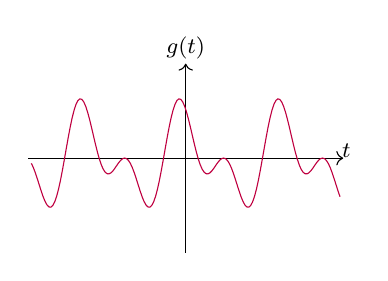
\begin{tikzpicture}
\begin{scope}[scale=0.4,yshift=-1cm]
	\draw[->] (-5,0)-- (5,0);
%\draw (-0.3,-0.3) node {0};
\draw[->] (0,-3)-- (0,3);
\draw (5.1,0.25) node {\footnotesize{$t$}};
\draw (0,3.5) node {\footnotesize{$g(t)$}};
%\draw (4.5,-0.3) node {1};

\draw[domain=-4.9:4.9,color=purple,samples=160] plot (\x,{2*(0.55*cos(2*\x r)+ 0.45*cos(2*2*(\x+3.14/12) r))});
\end{scope}
	\end{tikzpicture}
\end{center}

\column{60 mm}



\vspace{0.3cm}
\only<1>{
\begin{center}
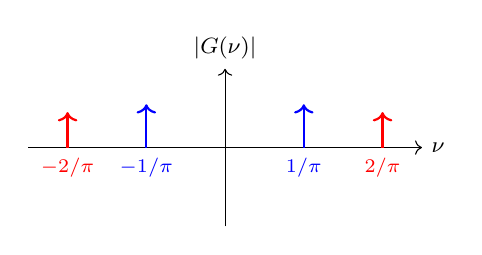
\begin{tikzpicture}
\draw[->] (-2.5,0)--(2.5,0) node[right]{\footnotesize{$\nu$}};
\draw[->] (0,-1)--(0,1) node[above]{\footnotesize{$|G(\nu)|$}};
\draw[->,blue,thick] (-1,0) node[below]{\scriptsize $-1/\pi$}--(-1,0.55) ;
\draw[->,blue,thick] (1,0) node[below]{\scriptsize $1/\pi$}--(1,0.55) ;
\draw[->,red,thick] (-2,0) node[below]{\scriptsize $-2/\pi$}--(-2,0.45) ;
\draw[->,red,thick] (2,0) node[below]{\scriptsize $2/\pi$}--(2,0.45) ;
\end{tikzpicture}
\end{center}
}

\only<2->{
\begin{center}
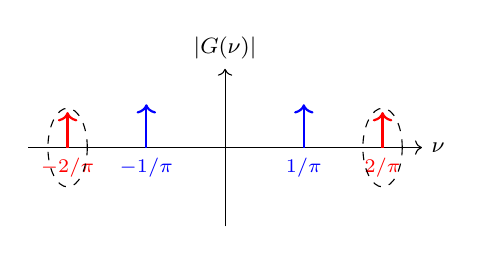
\begin{tikzpicture}
\draw[->] (-2.5,0)--(2.5,0) node[right]{\footnotesize{$\nu$}};
\draw[->] (0,-1)--(0,1) node[above]{\footnotesize{$|G(\nu)|$}};
\draw[->,blue,thick] (-1,0) node[below]{\scriptsize $-1/\pi$}--(-1,0.55) ;
\draw[->,blue,thick] (1,0) node[below]{\scriptsize $1/\pi$}--(1,0.55) ;
\draw[->,red,thick] (-2,0) node[below]{\scriptsize $-2/\pi$}--(-2,0.45) ;
\draw[->,red,thick] (2,0) node[below]{\scriptsize $2/\pi$}--(2,0.45) ;
\draw[dashed] (-2,0) ellipse (0.25 and 0.5) ;
\draw[dashed] (2,0) ellipse (0.25 and 0.5) ;
\end{tikzpicture}
\end{center}
}
\end{columns}
\vspace{0.3cm}
\only<2->{
Fréquence maximale : $2/\pi$ $\rightarrow$  $\nu_e > 2/\pi$
}
\end{frame}




\begin{frame}
\frametitle{\'Echantillonnage: exemple}
Dans les faits, respecter Shannon strictement est un peu limite...\\

\vspace{0.5cm}
\begin{columns}
\column{60mm}
\begin{center}
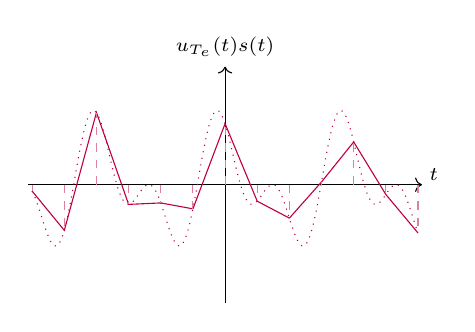
\begin{tikzpicture}
\begin{scope}[scale=0.5]
	\draw[->] (-5,0)-- (5,0);
%\draw (-0.3,-0.3) node {0};
\draw[->] (0,-3)-- (0,3);
\draw (5.3,0.25) node {\scriptsize $t$};
\draw (0,3.5) node {\scriptsize $u_{T_{e}}(t)s(t)$};
%\draw (4.5,-0.3) node {1};

\draw[domain=-4.9:4.9,color=purple,samples=13] plot (\x,{2*(0.55*cos(2*\x r)+ 0.45*cos(2*2*(\x+3.14/12) r))}); %0.6125 between each 

\draw[dotted,domain=-4.9:4.9,color=purple,samples=160] plot (\x,{2*(0.55*cos(2*\x r)+ 0.45*cos(2*2*(\x+3.14/12) r))});

\draw[dashed,domain=-4.9:4.9,color=purple!50!white,samples=13] plot[ycomb] (\x,{2*(0.55*cos(2*\x r)+ 0.45*cos(2*2*(\x+3.14/12) r))});

\end{scope}
\end{tikzpicture}
$\nu_e = 2 \nu_max$
\end{center}

\column{60mm}
\only<2>{
\begin{center}
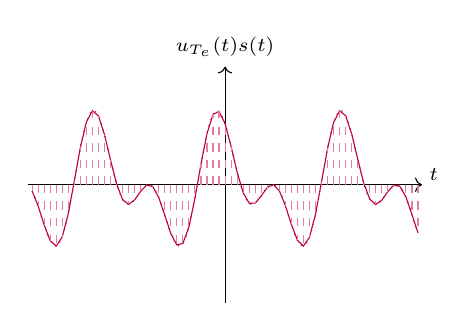
\begin{tikzpicture}
\begin{scope}[scale=0.5]
	\draw[->] (-5,0)-- (5,0);
%\draw (-0.3,-0.3) node {0};
\draw[->] (0,-3)-- (0,3);
\draw (5.3,0.25) node {\scriptsize $t$};
\draw (0,3.5) node {\scriptsize $u_{T_{e}}(t)s(t)$};
%\draw (4.5,-0.3) node {1};

\draw[domain=-4.9:4.9,color=purple,samples=65] plot (\x,{2*(0.55*cos(2*\x r)+ 0.45*cos(2*2*(\x+3.14/12) r))}); %0.6125 between each 

\draw[dotted,domain=-4.9:4.9,color=purple,samples=160] plot (\x,{2*(0.55*cos(2*\x r)+ 0.45*cos(2*2*(\x+3.14/12) r))});

\draw[dashed,domain=-4.9:4.9,color=purple!50!white,samples=65] plot[ycomb] (\x,{2*(0.55*cos(2*\x r)+ 0.45*cos(2*2*(\x+3.14/12) r))});

\end{scope}
\end{tikzpicture}
$\nu_e = 10 \nu_{max}$
\end{center}
}
\end{columns}
\only<2>{
\vspace{0.3cm}
\begin{block}{}
On prend plutôt $\nu_e > 5 \nu_{max}$ voire $\nu_e > 10 \nu_{max}$
\end{block}
}
\end{frame}

\begin{frame}
\frametitle{Impact de l'échantillonnage sur le spectre}

Il va nous falloir le spectre de \[u_{T_e}(t) \sum_{n = -\infty}^{\infty} \delta(t-nT_e))\]
\\
\vspace{0.2cm}
On sait que,
 \[  \sum_{n = -\infty}^{\infty} \delta(t-nT_e)) =  \frac{1}{T_e}\sum_{n = -\infty}^{\infty} \exp(j2\pi n \frac{t}{T_e}) \]
et donc,
 \[ TF(u_{T_e}(t)) =  TF(\frac{1}{T_e}\sum_{n = -\infty}^{\infty} \exp(j2\pi n \frac{t}{T_e})) =  \frac{1}{T_e}\sum_{n = -\infty}^{\infty} \delta(\nu - \frac{n}{T_e}) \] 
 

\end{frame}



\begin{frame}
\frametitle{Impact de l'échantillonnage sur le spectre}


\[ TF (\sum_{n = -\infty}^{\infty} g(t)\delta(t-nT_e)) = \frac{1}{T_e}\sum_{n = -\infty}^{\infty} G(\nu) \star \delta(\nu - \frac{n}{T_e}) \] 

Une propriété de la distribution de Dirac $\delta(x)$ est

\[\delta(x) \star f(x) = f(x) \]
Donc, 

\[ TF (\sum_{n = -\infty}^{\infty} g(t)\delta(t-nT_e)) = \frac{1}{T_e}\sum_{n = -\infty}^{\infty} G(\nu - \frac{n}{T_e}) \] 

\end{frame}

\begin{frame}
\frametitle{Impact de l'échantillonnage sur le spectre}

Donc  \[ TF(g_{T_e}(t)) =  \frac{1}{T_e}\sum_{n = -\infty}^{\infty} G(\nu - \frac{n}{T_e})) \]   

\vspace{0.1cm}
Représentons le spectre du signal échantillonné avec $\nu_e = 3/\pi$   
\begin{columns}[T]
\column{60mm}
\only<2->{
\begin{center}
\begin{tikzpicture}
\draw[->] (-2.5,0)--(2.5,0) node[right]{\footnotesize{$\nu$}};
\draw[->] (0,-1)--(0,1) node[above]{\footnotesize{$|G(\nu)|$}};
\draw[->,blue,thick] (-1/4,0) node[below]{\scriptsize $\frac{-1}{\pi}$}--(-1/4,0.55) ;
\draw[->,blue,thick] (1/4,0) node[below]{\scriptsize $\frac{1}{\pi}$}--(1/4,0.55) ;
\draw[->,red,thick] (-2/4,0) node[below]{\scriptsize $\frac{-2}{\pi}$}--(-2/4,0.45) ;
\draw[->,red,thick] (2/4,0) node[below]{\scriptsize $\frac{2}{\pi}$}--(2/4,0.45) ;
\end{tikzpicture}
\end{center}
}

\column{60mm}
\only<3>{
\begin{center}
\begin{tikzpicture}
\draw[->] (-2.5,0)--(2.5,0) node[right]{\footnotesize{$\nu$}};
\draw[->] (0,-1)--(0,1) node[above]{\footnotesize{$|G_{T_e}(\nu)|$}};
\draw[->,blue,thick] (-1/4,0) --(-1/4,0.55) ;
\draw[->,blue,thick] (1/4,0) --(1/4,0.55) ;
\draw[->,red,thick] (-2/4,0) --(-2/4,0.45) ;
\draw[->,red,thick] (2/4,0) --(2/4,0.45) ;%\draw[dashed] (-2,0) ellipse (0.25 and 0.5) ;
%\draw[dashed] (2,0) ellipse (0.25 and 0.5) ;
%\begin{scope}[xshift=1cm]
%\draw[->,blue,thick] (-1/4,0) --(-1/4,0.55) ;
%\draw[->,blue,thick] (1/4,0) --(1/4,0.55) ;
%\draw[->,blue,thick] (-2/4,0) --(-2/4,0.225) ;
%\draw[->,blue,thick] (2/4,0) --(2/4,0.225) ;
%\end{scope}
\end{tikzpicture}
\scriptsize{$n=0$}
\end{center}
}

\only<4>{
\begin{center}
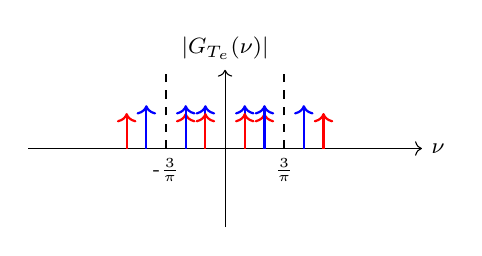
\begin{tikzpicture}
\draw[->] (-2.5,0)--(2.5,0) node[right]{\footnotesize{$\nu$}};
\draw[->] (0,-1)--(0,1) node[above]{\footnotesize{$|G_{T_e}(\nu)|$}};
\draw[->,blue,thick] (-1/4,0) --(-1/4,0.55) ;
\draw[->,blue,thick] (1/4,0) --(1/4,0.55) ;
\draw[->,red,thick] (-2/4,0) --(-2/4,0.45) ;
\draw[->,red,thick] (2/4,0) --(2/4,0.45) ;%\draw[dashed] (-2,0) ellipse (0.25 and 0.5) ;
%\draw[dashed] (2,0) ellipse (0.25 and 0.5) ;
\begin{scope}[xshift=0.75cm]
\draw[->,blue,thick] (-1/4,0) --(-1/4,0.55) ;
\draw[->,blue,thick] (1/4,0) --(1/4,0.55) ;
\draw[->,red,thick] (-2/4,0) --(-2/4,0.45) ;
\draw[->,red,thick] (2/4,0) --(2/4,0.45) ;
\draw[dashed,black,thick] (0,0) node[below]{\scriptsize{$\frac{3}{\pi}$}} --(0,1) ;
\end{scope}

\begin{scope}[xshift=-0.75cm]
\draw[->,blue,thick] (-1/4,0) --(-1/4,0.55) ;
\draw[->,blue,thick] (1/4,0) --(1/4,0.55) ;
\draw[->,red,thick] (-2/4,0) --(-2/4,0.45) ;
\draw[->,red,thick] (2/4,0) --(2/4,0.45) ;
\draw[dashed,black,thick] (0,0) node[below]{\scriptsize{-$\frac{3}{\pi}$}} --(0,1) ;
\end{scope}
\end{tikzpicture}
\scriptsize{$n=0, \pm 1$}
\end{center}
}

\only<5>{
\begin{center}
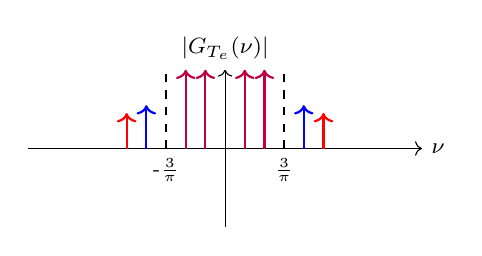
\begin{tikzpicture}
\draw[->] (-2.5,0)--(2.5,0) node[right]{\footnotesize{$\nu$}};
\draw[->] (0,-1)--(0,1) node[above]{\footnotesize{$|G_{T_e}(\nu)|$}};
\draw[->,purple,thick] (-1/4,0) --(-1/4,0.55+0.45) ;
\draw[->,purple,thick] (1/4,0) --(1/4,0.55+0.45) ;
\draw[->,purple,thick] (-2/4,0) --(-2/4,0.45+0.55) ;
\draw[->,purple,thick] (2/4,0) --(2/4,0.45+0.55) ;%\draw[dashed] (-2,0) ellipse (0.25 and 0.5) ;
%\draw[dashed] (2,0) ellipse (0.25 and 0.5) ;
\begin{scope}[xshift=0.75cm]
%\draw[->,blue,thick] (-1/4,0) --(-1/4,0.55) ;
\draw[->,blue,thick] (1/4,0) --(1/4,0.55) ;
%\draw[->,red,thick] (-2/4,0) --(-2/4,0.45) ;
\draw[->,red,thick] (2/4,0) --(2/4,0.45) ;
\draw[dashed,black,thick] (0,0) node[below]{\scriptsize{$\frac{3}{\pi}$}} --(0,1) ;
\end{scope}

\begin{scope}[xshift=-0.75cm]
\draw[->,blue,thick] (-1/4,0) --(-1/4,0.55) ;
%\draw[->,blue,thick] (1/4,0) --(1/4,0.55) ;
\draw[->,red,thick] (-2/4,0) --(-2/4,0.45) ;
%\draw[->,red,thick] (2/4,0) --(2/4,0.45) ;
\draw[dashed,black,thick] (0,0) node[below]{\scriptsize{-$\frac{3}{\pi}$}} --(0,1) ;
\end{scope}
\end{tikzpicture}
\scriptsize{$n=0, \pm 1$}
\end{center}
}

\only<6>{
\begin{center}
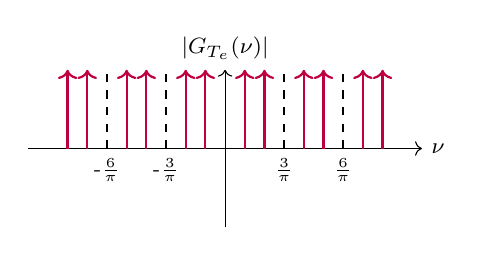
\begin{tikzpicture}
\draw[->] (-2.5,0)--(2.5,0) node[right]{\footnotesize{$\nu$}};
\draw[->] (0,-1)--(0,1) node[above]{\footnotesize{$|G_{T_e}(\nu)|$}};
\draw[->,purple,thick] (-1/4,0) --(-1/4,0.55+0.45) ;
\draw[->,purple,thick] (1/4,0) --(1/4,0.55+0.45) ;
\draw[->,purple,thick] (-2/4,0) --(-2/4,0.45+0.55) ;
\draw[->,purple,thick] (2/4,0) --(2/4,0.45+0.55) ;%\draw[dashed] (-2,0) ellipse (0.25 and 0.5) ;
%\draw[dashed] (2,0) ellipse (0.25 and 0.5) ;


\begin{scope}[xshift=0.75cm]
%\draw[->,blue,thick] (-1/4,0) --(-1/4,0.55) ;
\draw[->,purple,thick] (1/4,0) --(1/4,0.55+0.45) ;
%\draw[->,red,thick] (-2/4,0) --(-2/4,0.45) ;
\draw[->,purple,thick] (2/4,0) --(2/4,0.45+0.55) ;
\draw[dashed,black,thick] (0,0) node[below]{\scriptsize{$\frac{3}{\pi}$}} --(0,1) ;
\end{scope}

\begin{scope}[xshift=-0.75cm]
\draw[->,purple,thick] (-1/4,0) --(-1/4,0.55+0.45) ;
%\draw[->,blue,thick] (1/4,0) --(1/4,0.55) ;
\draw[->,purple,thick] (-2/4,0) --(-2/4,0.45+0.55) ;
%\draw[->,red,thick] (2/4,0) --(2/4,0.45) ;
\draw[dashed,black,thick] (0,0) node[below]{\scriptsize{-$\frac{3}{\pi}$}} --(0,1) ;
\end{scope}

\begin{scope}[xshift=1.5cm]
%\draw[->,blue,thick] (-1/4,0) --(-1/4,0.55) ;
\draw[->,purple,thick] (1/4,0) --(1/4,0.55+0.45) ;
%\draw[->,red,thick] (-2/4,0) --(-2/4,0.45) ;
\draw[->,purple,thick] (2/4,0) --(2/4,0.45+0.55) ;
\draw[dashed,black,thick] (0,0) node[below]{\scriptsize{$\frac{6}{\pi}$}} --(0,1) ;
\end{scope}

\begin{scope}[xshift=-1.5cm]
\draw[->,purple,thick] (-1/4,0) --(-1/4,0.55+0.45) ;
%\draw[->,blue,thick] (1/4,0) --(1/4,0.55) ;
\draw[->,purple,thick] (-2/4,0) --(-2/4,0.45+0.55) ;
%\draw[->,red,thick] (2/4,0) --(2/4,0.45) ;
\draw[dashed,black,thick] (0,0) node[below]{\scriptsize{-$\frac{6}{\pi}$}} --(0,1) ;
\end{scope}
\end{tikzpicture}
\scriptsize{$n=0, \pm 1, \pm 2,...$}
\end{center}
}


\end{columns}

\only<4->{
\begin{block}{}
On note que la fréquence minimale et maximale des répliques adjacentes se superposent $\rightarrow$ spectre déformé
\end{block}
}

\end{frame}

\begin{frame}
\frametitle{Impact de l'échantillonnage sur le spectre}
Représentons le spectre du signal échantillonné avec $\nu_e = 3/\pi$
\begin{columns}
\column{60mm}
\begin{center}
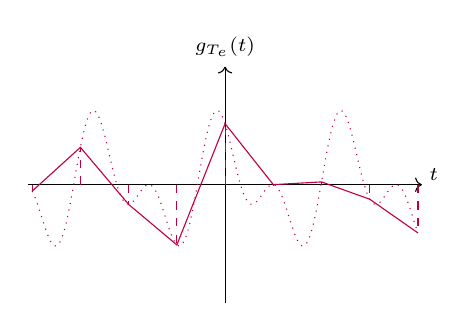
\begin{tikzpicture}
\begin{scope}[scale=0.5]
	\draw[->] (-5,0)-- (5,0);
%\draw (-0.3,-0.3) node {0};
\draw[->] (0,-3)-- (0,3);
\draw (5.3,0.25) node {\scriptsize $t$};
\draw (0,3.5) node {\scriptsize $g_{T_{e}}(t)$};
%\draw (4.5,-0.3) node {1};

\draw[domain=-4.9:4.9,color=purple,samples=9] plot (\x,{2*(0.55*cos(2*\x r)+ 0.45*cos(2*2*(\x+3.14/12) r))}); %0.6125 between each 

\draw[dotted,domain=-4.9:4.9,color=purple,samples=160] plot (\x,{2*(0.55*cos(2*\x r)+ 0.45*cos(2*2*(\x+3.14/12) r))});

\draw[dashed,domain=-4.9:4.9,color=purple,samples=9] plot[ycomb] (\x,{2*(0.55*cos(2*\x r)+ 0.45*cos(2*2*(\x+3.14/12) r))});

\end{scope}
\end{tikzpicture}
\end{center}

\column{60mm}
\begin{center}
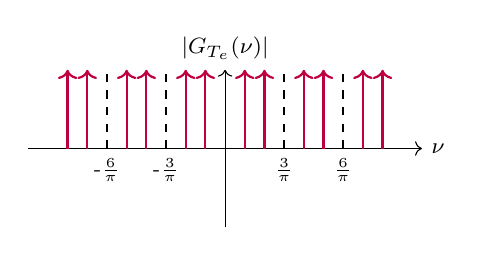
\begin{tikzpicture}
\draw[->] (-2.5,0)--(2.5,0) node[right]{\footnotesize{$\nu$}};
\draw[->] (0,-1)--(0,1) node[above]{\footnotesize{$|G_{T_e}(\nu)|$}};
\draw[->,purple,thick] (-1/4,0) --(-1/4,0.55+0.45) ;
\draw[->,purple,thick] (1/4,0) --(1/4,0.55+0.45) ;
\draw[->,purple,thick] (-2/4,0) --(-2/4,0.45+0.55) ;
\draw[->,purple,thick] (2/4,0) --(2/4,0.45+0.55) ;%\draw[dashed] (-2,0) ellipse (0.25 and 0.5) ;
%\draw[dashed] (2,0) ellipse (0.25 and 0.5) ;


\begin{scope}[xshift=0.75cm]
%\draw[->,blue,thick] (-1/4,0) --(-1/4,0.55) ;
\draw[->,purple,thick] (1/4,0) --(1/4,0.55+0.45) ;
%\draw[->,red,thick] (-2/4,0) --(-2/4,0.45) ;
\draw[->,purple,thick] (2/4,0) --(2/4,0.45+0.55) ;
\draw[dashed,black,thick] (0,0) node[below]{\scriptsize{$\frac{3}{\pi}$}} --(0,1) ;
\end{scope}

\begin{scope}[xshift=-0.75cm]
\draw[->,purple,thick] (-1/4,0) --(-1/4,0.55+0.45) ;
%\draw[->,blue,thick] (1/4,0) --(1/4,0.55) ;
\draw[->,purple,thick] (-2/4,0) --(-2/4,0.45+0.55) ;
%\draw[->,red,thick] (2/4,0) --(2/4,0.45) ;
\draw[dashed,black,thick] (0,0) node[below]{\scriptsize{-$\frac{3}{\pi}$}} --(0,1) ;
\end{scope}

\begin{scope}[xshift=1.5cm]
%\draw[->,blue,thick] (-1/4,0) --(-1/4,0.55) ;
\draw[->,purple,thick] (1/4,0) --(1/4,0.55+0.45) ;
%\draw[->,red,thick] (-2/4,0) --(-2/4,0.45) ;
\draw[->,purple,thick] (2/4,0) --(2/4,0.45+0.55) ;
\draw[dashed,black,thick] (0,0) node[below]{\scriptsize{$\frac{6}{\pi}$}} --(0,1) ;
\end{scope}

\begin{scope}[xshift=-1.5cm]
\draw[->,purple,thick] (-1/4,0) --(-1/4,0.55+0.45) ;
%\draw[->,blue,thick] (1/4,0) --(1/4,0.55) ;
\draw[->,purple,thick] (-2/4,0) --(-2/4,0.45+0.55) ;
%\draw[->,red,thick] (2/4,0) --(2/4,0.45) ;
\draw[dashed,black,thick] (0,0) node[below]{\scriptsize{-$\frac{6}{\pi}$}} --(0,1) ;
\end{scope}
\end{tikzpicture}
\scriptsize{$n=0, \pm 1, \pm 2,...$}
\end{center}

\end{columns}

\begin{block}{}
Le signal est ici sous-échantillonné... Les spectres des répliques se superposent
\end{block}
\end{frame}


\begin{frame}
\frametitle{Impact de l'échantillonnage sur le spectre}

Donc  \[ TF(g_{T_e}(t)) =  \frac{1}{T_e}\sum_{n = -\infty}^{\infty} G(\nu - \frac{n}{T_e})) \]   

\vspace{0.1cm}
Représentons le spectre du signal échantillonné avec $\nu_e = 4/\pi$   
\begin{columns}[T]
\column{60mm}
\only<2->{
\begin{center}
\begin{tikzpicture}
\draw[->] (-2.5,0)--(2.5,0) node[right]{\footnotesize{$\nu$}};
\draw[->] (0,-1)--(0,1) node[above]{\footnotesize{$|G(\nu)|$}};
\draw[->,blue,thick] (-1/4,0) node[below]{\scriptsize $\frac{-1}{\pi}$}--(-1/4,0.55) ;
\draw[->,blue,thick] (1/4,0) node[below]{\scriptsize $\frac{1}{\pi}$}--(1/4,0.55) ;
\draw[->,red,thick] (-2/4,0) node[below]{\scriptsize $\frac{-2}{\pi}$}--(-2/4,0.45) ;
\draw[->,red,thick] (2/4,0) node[below]{\scriptsize $\frac{2}{\pi}$}--(2/4,0.45) ;
\end{tikzpicture}
\end{center}
}

\column{60mm}
\only<3>{
\begin{center}
\begin{tikzpicture}
\draw[->] (-2.5,0)--(2.5,0) node[right]{\footnotesize{$\nu$}};
\draw[->] (0,-1)--(0,1) node[above]{\footnotesize{$|G(\nu)|$}};
\draw[->,blue,thick] (-1/4,0) --(-1/4,0.55) ;
\draw[->,blue,thick] (1/4,0) --(1/4,0.55) ;
\draw[->,red,thick] (-2/4,0) --(-2/4,0.45) ;
\draw[->,red,thick] (2/4,0) --(2/4,0.45) ;%\draw[dashed] (-2,0) ellipse (0.25 and 0.5) ;
%\draw[dashed] (2,0) ellipse (0.25 and 0.5) ;
%\begin{scope}[xshift=1cm]
%\draw[->,blue,thick] (-1/4,0) --(-1/4,0.55) ;
%\draw[->,blue,thick] (1/4,0) --(1/4,0.55) ;
%\draw[->,blue,thick] (-2/4,0) --(-2/4,0.225) ;
%\draw[->,blue,thick] (2/4,0) --(2/4,0.225) ;
%\end{scope}
\end{tikzpicture}
\scriptsize{$n=0$}
\end{center}
}

\only<4>{
\begin{center}
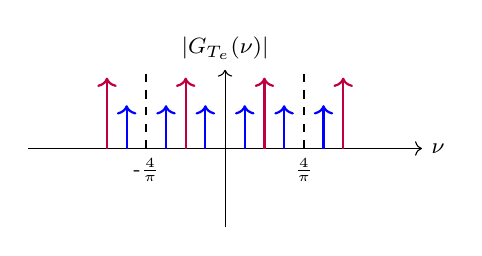
\begin{tikzpicture}
\draw[->] (-2.5,0)--(2.5,0) node[right]{\footnotesize{$\nu$}};
\draw[->] (0,-1)--(0,1) node[above]{\footnotesize{$|G_{T_e}(\nu)|$}};
\draw[->,blue,thick] (-1/4,0) --(-1/4,0.55) ;
\draw[->,blue,thick] (1/4,0) --(1/4,0.55) ;
%\draw[->,purple,thick] (-2/4,0) --(-2/4,0.225) ;
%\draw[->,purple,thick] (2/4,0) --(2/4,0.225) ;%\draw[dashed] (-2,0) ellipse (0.25 and 0.5) ;
%\draw[dashed] (2,0) ellipse (0.25 and 0.5) ;
\begin{scope}[xshift=1cm]
\draw[->,blue,thick] (-1/4,0) --(-1/4,0.55) ;
\draw[->,blue,thick] (1/4,0) --(1/4,0.55) ;
\draw[->,purple,thick] (-2/4,0) --(-2/4,0.9) ;
\draw[->,purple,thick] (2/4,0) --(2/4,0.9) ;
\draw[dashed,black,thick] (0,0) node[below]{\scriptsize{$\frac{4}{\pi}$}} --(0,1) ;
\end{scope}

\begin{scope}[xshift=-1cm]
\draw[->,blue,thick] (-1/4,0) --(-1/4,0.55) ;
\draw[->,blue,thick] (1/4,0) --(1/4,0.55) ;
\draw[->,purple,thick] (-2/4,0) --(-2/4,0.9) ;
\draw[->,purple,thick] (2/4,0) --(2/4,0.9) ;
\draw[dashed,black,thick] (0,0) node[below]{\scriptsize{-$\frac{4}{\pi}$}} --(0,1) ;
\end{scope}
\end{tikzpicture}
\scriptsize{$n=0, \pm 1$}
\end{center}
}

\only<5->{
\begin{center}
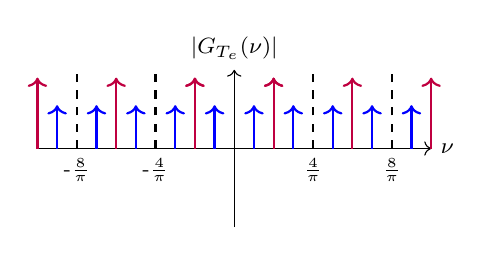
\begin{tikzpicture}
\draw[->] (-2.5,0)--(2.5,0) node[right]{\footnotesize{$\nu$}};
\draw[->] (0,-1)--(0,1) node[above]{\footnotesize{$|G_{T_e}(\nu)|$}};
\draw[->,blue,thick] (-1/4,0) --(-1/4,0.55) ;
\draw[->,blue,thick] (1/4,0) --(1/4,0.55) ;
\draw[->,purple,thick] (-2/4,0) --(-2/4,0.9) ;
\draw[->,purple,thick] (2/4,0) --(2/4,0.9) ;%\draw[dashed] (-2,0) ellipse (0.25 and 0.5) ;
%\draw[dashed] (2,0) ellipse (0.25 and 0.5) ;
\begin{scope}[xshift=1cm]
\draw[->,blue,thick] (-1/4,0) --(-1/4,0.55) ;
\draw[->,blue,thick] (1/4,0) --(1/4,0.55) ;
\draw[->,purple,thick] (-2/4,0) --(-2/4,0.9) ;
\draw[->,purple,thick] (2/4,0) --(2/4,0.9) ;
\draw[dashed,black,thick] (0,0) node[below]{\scriptsize{$\frac{4}{\pi}$}} --(0,1) ;
\end{scope}

\begin{scope}[xshift=-1cm]
\draw[->,blue,thick] (-1/4,0) --(-1/4,0.55) ;
\draw[->,blue,thick] (1/4,0) --(1/4,0.55) ;
\draw[->,purple,thick] (-2/4,0) --(-2/4,0.9) ;
\draw[->,purple,thick] (2/4,0) --(2/4,0.9) ;
\draw[dashed,black,thick] (0,0) node[below]{\scriptsize{-$\frac{4}{\pi}$}} --(0,1) ;
\end{scope}

\begin{scope}[xshift=2cm]
\draw[->,blue,thick] (-1/4,0) --(-1/4,0.55) ;
\draw[->,blue,thick] (1/4,0) --(1/4,0.55) ;
%\draw[->,purple,thick] (-2/4,0) --(-2/4,0.9) ;
\draw[->,purple,thick] (2/4,0) --(2/4,0.9) ;
\draw[dashed,black,thick] (0,0) node[below]{\scriptsize{$\frac{8}{\pi}$}} --(0,1) ;
\end{scope}

\begin{scope}[xshift=-2cm]
\draw[->,blue,thick] (-1/4,0) --(-1/4,0.55) ;
\draw[->,blue,thick] (1/4,0) --(1/4,0.55) ;
\draw[->,purple,thick] (-2/4,0) --(-2/4,0.9) ;
%\draw[->,purple,thick] (2/4,0) --(2/4,0.55) ;
\draw[dashed,black,thick] (0,0) node[below]{\scriptsize{-$\frac{8}{\pi}$}} --(0,1) ;
\end{scope}
\end{tikzpicture}
\scriptsize{$n=0,\pm 1,\pm 2...$}
\end{center}
}


\end{columns}

\only<4->{
\begin{block}{}
On note que la fréquence minimale et maximale des répliques adjacentes se superposent $\rightarrow$ spectre déformé
\end{block}
}

\end{frame}

\begin{frame}
\frametitle{Impact de l'échantillonnage sur le spectre}
\vspace{0.1cm}
Représentons le spectre du signal échantillonné avec $\nu_e = 4/\pi$
\begin{columns}
\column{60mm}
\begin{center}
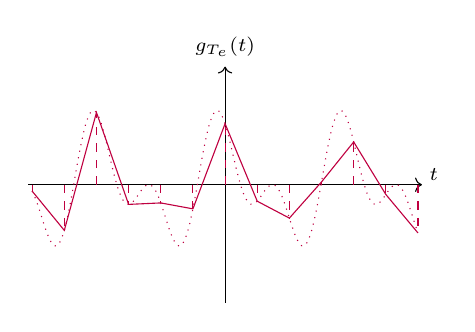
\begin{tikzpicture}
\begin{scope}[scale=0.5]
	\draw[->] (-5,0)-- (5,0);
%\draw (-0.3,-0.3) node {0};
\draw[->] (0,-3)-- (0,3);
\draw (5.3,0.25) node {\scriptsize $t$};
\draw (0,3.5) node {\scriptsize $g_{T_{e}}(t)$};
%\draw (4.5,-0.3) node {1};

\draw[domain=-4.9:4.9,color=purple,samples=13] plot (\x,{2*(0.55*cos(2*\x r)+ 0.45*cos(2*2*(\x+3.14/12) r))}); %0.6125 between each 

\draw[dotted,domain=-4.9:4.9,color=purple,samples=160] plot (\x,{2*(0.55*cos(2*\x r)+ 0.45*cos(2*2*(\x+3.14/12) r))});

\draw[dashed,domain=-4.9:4.9,color=purple,samples=13] plot[ycomb] (\x,{2*(0.55*cos(2*\x r)+ 0.45*cos(2*2*(\x+3.14/12) r))});

\end{scope}
\end{tikzpicture}
$\nu_e = 4/\pi$
\end{center}
\column{60mm}
\begin{center}
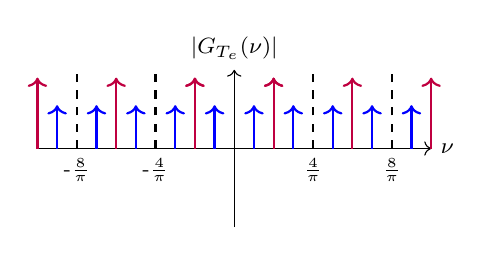
\begin{tikzpicture}
\draw[->] (-2.5,0)--(2.5,0) node[right]{\footnotesize{$\nu$}};
\draw[->] (0,-1)--(0,1) node[above]{\footnotesize{$|G_{T_e}(\nu)|$}};
\draw[->,blue,thick] (-1/4,0) --(-1/4,0.55) ;
\draw[->,blue,thick] (1/4,0) --(1/4,0.55) ;
\draw[->,purple,thick] (-2/4,0) --(-2/4,0.9) ;
\draw[->,purple,thick] (2/4,0) --(2/4,0.9) ;%\draw[dashed] (-2,0) ellipse (0.25 and 0.5) ;
%\draw[dashed] (2,0) ellipse (0.25 and 0.5) ;
\begin{scope}[xshift=1cm]
\draw[->,blue,thick] (-1/4,0) --(-1/4,0.55) ;
\draw[->,blue,thick] (1/4,0) --(1/4,0.55) ;
\draw[->,purple,thick] (-2/4,0) --(-2/4,0.9) ;
\draw[->,purple,thick] (2/4,0) --(2/4,0.9) ;
\draw[dashed,black,thick] (0,0) node[below]{\scriptsize{$\frac{4}{\pi}$}} --(0,1) ;
\end{scope}

\begin{scope}[xshift=-1cm]
\draw[->,blue,thick] (-1/4,0) --(-1/4,0.55) ;
\draw[->,blue,thick] (1/4,0) --(1/4,0.55) ;
\draw[->,purple,thick] (-2/4,0) --(-2/4,0.9) ;
\draw[->,purple,thick] (2/4,0) --(2/4,0.9) ;
\draw[dashed,black,thick] (0,0) node[below]{\scriptsize{-$\frac{4}{\pi}$}} --(0,1) ;
\end{scope}

\begin{scope}[xshift=2cm]
\draw[->,blue,thick] (-1/4,0) --(-1/4,0.55) ;
\draw[->,blue,thick] (1/4,0) --(1/4,0.55) ;
%\draw[->,purple,thick] (-2/4,0) --(-2/4,0.9) ;
\draw[->,purple,thick] (2/4,0) --(2/4,0.9) ;
\draw[dashed,black,thick] (0,0) node[below]{\scriptsize{$\frac{8}{\pi}$}} --(0,1) ;
\end{scope}

\begin{scope}[xshift=-2cm]
\draw[->,blue,thick] (-1/4,0) --(-1/4,0.55) ;
\draw[->,blue,thick] (1/4,0) --(1/4,0.55) ;
\draw[->,purple,thick] (-2/4,0) --(-2/4,0.9) ;
%\draw[->,purple,thick] (2/4,0) --(2/4,0.55) ;
\draw[dashed,black,thick] (0,0) node[below]{\scriptsize{-$\frac{8}{\pi}$}} --(0,1) ;
\end{scope}
\end{tikzpicture}
\end{center}
\end{columns}
\end{frame}

%%%%%%%%%%%%%%%%%%%%%%%%%%%%%%%%%%%%%%%%%%%%%%%%%%%%%%%%%%%%%%%%%%%%%%%%%%
\begin{frame}
\frametitle{Impact de l'échantillonnage sur le spectre}

Donc  \[ TF(g_{T_e}(t)) =  \frac{1}{T_e}\sum_{n = -\infty}^{\infty} G(\nu - \frac{n}{T_e})) \]   

\vspace{0.1cm}
Représentons le spectre du signal échantillonné avec $\nu_e = 5/\pi$   
\begin{columns}[T]
\column{60mm}
\only<2->{
\begin{center}
\begin{tikzpicture}
\draw[->] (-2.5,0)--(2.5,0) node[right]{\footnotesize{$\nu$}};
\draw[->] (0,-1)--(0,1) node[above]{\footnotesize{$|G(\nu)|$}};
\draw[->,blue,thick] (-1/4,0) node[below]{\scriptsize $\frac{-1}{\pi}$}--(-1/4,0.55) ;
\draw[->,blue,thick] (1/4,0) node[below]{\scriptsize $\frac{1}{\pi}$}--(1/4,0.55) ;
\draw[->,red,thick] (-2/4,0) node[below]{\scriptsize $\frac{-2}{\pi}$}--(-2/4,0.45) ;
\draw[->,red,thick] (2/4,0) node[below]{\scriptsize $\frac{2}{\pi}$}--(2/4,0.45) ;
\end{tikzpicture}
\end{center}
}

\column{60mm}
\only<3>{
\begin{center}
\begin{tikzpicture}
\draw[->] (-2.5,0)--(2.5,0) node[right]{\footnotesize{$\nu$}};
\draw[->] (0,-1)--(0,1) node[above]{\footnotesize{$|G(\nu)|$}};
\draw[->,blue,thick] (-1/4,0) --(-1/4,0.55) ;
\draw[->,blue,thick] (1/4,0) --(1/4,0.55) ;
\draw[->,red,thick] (-2/4,0) --(-2/4,0.45) ;
\draw[->,red,thick] (2/4,0) --(2/4,0.45) ;%\draw[dashed] (-2,0) ellipse (0.25 and 0.5) ;
%\draw[dashed] (2,0) ellipse (0.25 and 0.5) ;
%\begin{scope}[xshift=1cm]
%\draw[->,blue,thick] (-1/4,0) --(-1/4,0.55) ;
%\draw[->,blue,thick] (1/4,0) --(1/4,0.55) ;
%\draw[->,blue,thick] (-2/4,0) --(-2/4,0.225) ;
%\draw[->,blue,thick] (2/4,0) --(2/4,0.225) ;
%\end{scope}
\end{tikzpicture}
\scriptsize{$n=0$}
\end{center}
}

\only<4>{
\begin{center}
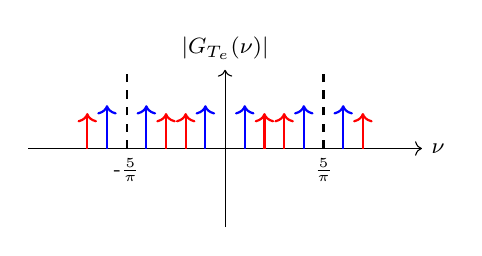
\begin{tikzpicture}
\draw[->] (-2.5,0)--(2.5,0) node[right]{\footnotesize{$\nu$}};
\draw[->] (0,-1)--(0,1) node[above]{\footnotesize{$|G_{T_e}(\nu)|$}};
\draw[->,blue,thick] (-1/4,0) --(-1/4,0.55) ;
\draw[->,blue,thick] (1/4,0) --(1/4,0.55) ;
\draw[->,red,thick] (-2/4,0) --(-2/4,0.45) ;
\draw[->,red,thick] (2/4,0) --(2/4,0.45) ;%\draw[dashed] (-2,0) ellipse (0.25 and 0.5) ;
%\draw[dashed] (2,0) ellipse (0.25 and 0.5) ;
\begin{scope}[xshift=1.25cm]
\draw[->,blue,thick] (-1/4,0) --(-1/4,0.55) ;
\draw[->,blue,thick] (1/4,0) --(1/4,0.55) ;
\draw[->,red,thick] (-2/4,0) --(-2/4,0.45) ;
\draw[->,red,thick] (2/4,0) --(2/4,0.45) ;
\draw[dashed,black,thick] (0,0) node[below]{\scriptsize{$\frac{5}{\pi}$}} --(0,1) ;
\end{scope}

\begin{scope}[xshift=-1.25cm]
\draw[->,blue,thick] (-1/4,0) --(-1/4,0.55) ;
\draw[->,blue,thick] (1/4,0) --(1/4,0.55) ;
\draw[->,red,thick] (-2/4,0) --(-2/4,0.45) ;
\draw[->,red,thick] (2/4,0) --(2/4,0.45) ;
\draw[dashed,black,thick] (0,0) node[below]{\scriptsize{-$\frac{5}{\pi}$}} --(0,1) ;
\end{scope}
\end{tikzpicture}
\scriptsize{$n=0, \pm 1$}
\end{center}
}

\only<5->{
\begin{center}
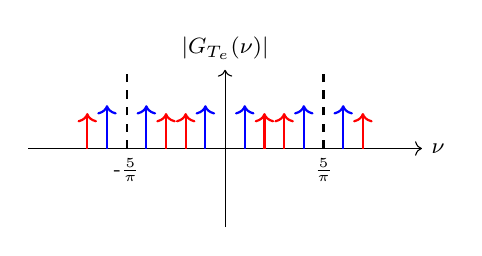
\begin{tikzpicture}
\draw[->] (-2.5,0)--(2.5,0) node[right]{\footnotesize{$\nu$}};
\draw[->] (0,-1)--(0,1) node[above]{\footnotesize{$|G_{T_e}(\nu)|$}};
\draw[->,blue,thick] (-1/4,0) --(-1/4,0.55) ;
\draw[->,blue,thick] (1/4,0) --(1/4,0.55) ;
\draw[->,red,thick] (-2/4,0) --(-2/4,0.45) ;
\draw[->,red,thick] (2/4,0) --(2/4,0.45) ;%\draw[dashed] (-2,0) ellipse (0.25 and 0.5) ;
%\draw[dashed] (2,0) ellipse (0.25 and 0.5) ;
\begin{scope}[xshift=1.25cm]
\draw[->,blue,thick] (-1/4,0) --(-1/4,0.55) ;
\draw[->,blue,thick] (1/4,0) --(1/4,0.55) ;
\draw[->,red,thick] (-2/4,0) --(-2/4,0.45) ;
\draw[->,red,thick] (2/4,0) --(2/4,0.45) ;
\draw[dashed,black,thick] (0,0) node[below]{\scriptsize{$\frac{5}{\pi}$}} --(0,1) ;
\end{scope}

\begin{scope}[xshift=-1.25cm]
\draw[->,blue,thick] (-1/4,0) --(-1/4,0.55) ;
\draw[->,blue,thick] (1/4,0) --(1/4,0.55) ;
\draw[->,red,thick] (-2/4,0) --(-2/4,0.45) ;
\draw[->,red,thick] (2/4,0) --(2/4,0.45) ;
\draw[dashed,black,thick] (0,0) node[below]{\scriptsize{-$\frac{5}{\pi}$}} --(0,1) ;
\end{scope}

%\begin{scope}[xshift=2cm]
%\draw[->,blue,thick] (-1/4,0) --(-1/4,0.55) ;
%\draw[->,blue,thick] (1/4,0) --(1/4,0.55) ;
%%\draw[->,purple,thick] (-2/4,0) --(-2/4,0.9) ;
%\draw[->,purple,thick] (2/4,0) --(2/4,0.9) ;
%\draw[dashed,black,thick] (0,0) node[below]{\scriptsize{$\frac{8}{\pi}$}} --(0,1) ;
%\end{scope}

%\begin{scope}[xshift=-2cm]
%\draw[->,blue,thick] (-1/4,0) --(-1/4,0.55) ;
%\draw[->,blue,thick] (1/4,0) --(1/4,0.55) ;
%\draw[->,purple,thick] (-2/4,0) --(-2/4,0.9) ;
%%\draw[->,purple,thick] (2/4,0) --(2/4,0.55) ;
%\draw[dashed,black,thick] (0,0) node[below]{\scriptsize{-$\frac{8}{\pi}$}} --(0,1) ;
%\end{scope}
\end{tikzpicture}
\scriptsize{$n=0,\pm 1,\pm 2...$}
\end{center}
}


\end{columns}

\only<4->{
\begin{block}{}
On note que la fréquence minimale et maximale des répliques adjacentes se superposent $\rightarrow$ spectre déformé
\end{block}
}

\end{frame}

\begin{frame}
\frametitle{Impact de l'échantillonnage sur le spectre}
\vspace{0.1cm}
Représentons le spectre du signal échantillonné avec $\nu_e = 5/\pi$
\begin{columns}
\column{60mm}
\begin{center}
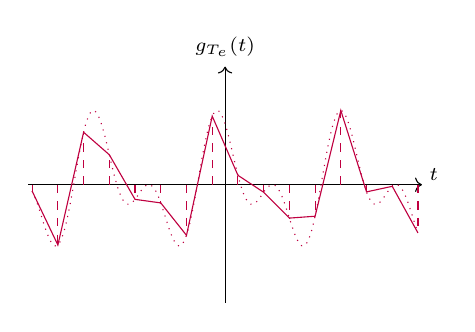
\begin{tikzpicture}
\begin{scope}[scale=0.5]
	\draw[->] (-5,0)-- (5,0);
%\draw (-0.3,-0.3) node {0};
\draw[->] (0,-3)-- (0,3);
\draw (5.3,0.25) node {\scriptsize $t$};
\draw (0,3.5) node {\scriptsize $g_{T_{e}}(t)$};
%\draw (4.5,-0.3) node {1};

\draw[domain=-4.9:4.9,color=purple,samples=16] plot (\x,{2*(0.55*cos(2*\x r)+ 0.45*cos(2*2*(\x+3.14/12) r))}); %0.6125 between each 

\draw[dotted,domain=-4.9:4.9,color=purple,samples=160] plot (\x,{2*(0.55*cos(2*\x r)+ 0.45*cos(2*2*(\x+3.14/12) r))});

\draw[dashed,domain=-4.9:4.9,color=purple,samples=16] plot[ycomb] (\x,{2*(0.55*cos(2*\x r)+ 0.45*cos(2*2*(\x+3.14/12) r))});

\end{scope}
\end{tikzpicture}
$\nu_e = 5/\pi$
\end{center}
\column{60mm}
\begin{center}
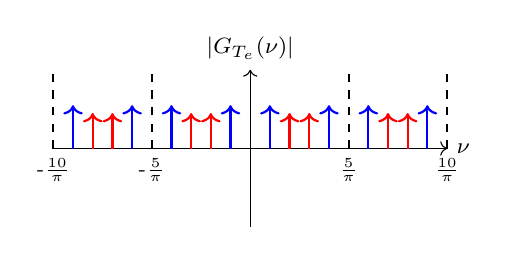
\begin{tikzpicture}
\draw[->] (-2.5,0)--(2.5,0) node[right]{\footnotesize{$\nu$}};
\draw[->] (0,-1)--(0,1) node[above]{\footnotesize{$|G_{T_e}(\nu)|$}};
\draw[->,blue,thick] (-1/4,0) --(-1/4,0.55) ;
\draw[->,blue,thick] (1/4,0) --(1/4,0.55) ;
\draw[->,red,thick] (-2/4,0) --(-2/4,0.45) ;
\draw[->,red,thick] (2/4,0) --(2/4,0.45) ;%\draw[dashed] (-2,0) ellipse (0.25 and 0.5) ;
%\draw[dashed] (2,0) ellipse (0.25 and 0.5) ;
\begin{scope}[xshift=1.25cm]
\draw[->,blue,thick] (-1/4,0) --(-1/4,0.55) ;
\draw[->,blue,thick] (1/4,0) --(1/4,0.55) ;
\draw[->,red,thick] (-2/4,0) --(-2/4,0.45) ;
\draw[->,red,thick] (2/4,0) --(2/4,0.45) ;
\draw[dashed,black,thick] (0,0) node[below]{\scriptsize{$\frac{5}{\pi}$}} --(0,1) ;
\end{scope}

\begin{scope}[xshift=-1.25cm]
\draw[->,blue,thick] (-1/4,0) --(-1/4,0.55) ;
\draw[->,blue,thick] (1/4,0) --(1/4,0.55) ;
\draw[->,red,thick] (-2/4,0) --(-2/4,0.45) ;
\draw[->,red,thick] (2/4,0) --(2/4,0.45) ;
\draw[dashed,black,thick] (0,0) node[below]{\scriptsize{-$\frac{5}{\pi}$}} --(0,1) ;
\end{scope}

\begin{scope}[xshift=2.5cm]
\draw[->,blue,thick] (-1/4,0) --(-1/4,0.55) ;
%\draw[->,blue,thick] (1/4,0) --(1/4,0.55) ;
\draw[->,red,thick] (-2/4,0) --(-2/4,0.45) ;
%\draw[->,purple,thick] (2/4,0) --(2/4,0.45) ;
\draw[dashed,black,thick] (0,0) node[below]{\scriptsize{$\frac{10}{\pi}$}} --(0,1) ;
\end{scope}

\begin{scope}[xshift=-2.5cm]
%\draw[->,blue,thick] (-1/4,0) --(-1/4,0.55) ;
\draw[->,blue,thick] (1/4,0) --(1/4,0.55) ;
%\draw[->,red,thick] (-2/4,0) --(-2/4,0.45) ;
\draw[->,red,thick] (2/4,0) --(2/4,0.45) ;
\draw[dashed,black,thick] (0,0) node[below]{\scriptsize{-$\frac{10}{\pi}$}} --(0,1) ;
\end{scope}
\end{tikzpicture}
\end{center}
\end{columns}
\end{frame}


%%%%%%%%%%%%%%%%%%%%%%%%%%%%%%%%%%%%%%%%%%%%%%%%%%%%%%%%%%%%%%%%%%%%%%%%%%%
\begin{frame}
\frametitle{Impact de l'échantillonnage sur le spectre}
\begin{columns}[T]
\column{40mm}
\begin{center}
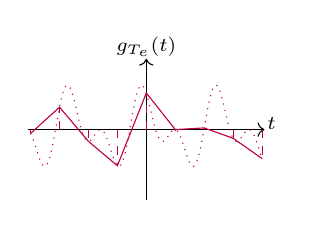
\begin{tikzpicture}
\begin{scope}[scale=0.3]
	\draw[->] (-5,0)-- (5,0);
%\draw (-0.3,-0.3) node {0};
\draw[->] (0,-3)-- (0,3);
\draw (5.3,0.25) node {\scriptsize $t$};
\draw (0,3.5) node {\scriptsize $g_{T_{e}}(t)$};
%\draw (4.5,-0.3) node {1};

\draw[domain=-4.9:4.9,color=purple,samples=9] plot (\x,{2*(0.55*cos(2*\x r)+ 0.45*cos(2*2*(\x+3.14/12) r))}); %0.6125 between each 

\draw[dotted,domain=-4.9:4.9,color=purple,samples=160] plot (\x,{2*(0.55*cos(2*\x r)+ 0.45*cos(2*2*(\x+3.14/12) r))});

\draw[dashed,domain=-4.9:4.9,color=purple,samples=9] plot[ycomb] (\x,{2*(0.55*cos(2*\x r)+ 0.45*cos(2*2*(\x+3.14/12) r))});

\end{scope}
\end{tikzpicture}
\end{center}

\begin{center}
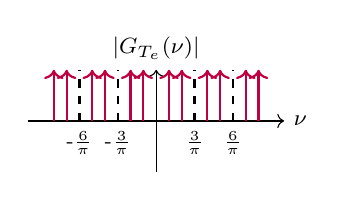
\begin{tikzpicture}
\begin{scope}[scale=0.65]
\draw[->] (-2.5,0)--(2.5,0) node[right]{\footnotesize{$\nu$}};
\draw[->] (0,-1)--(0,1) node[above]{\footnotesize{$|G_{T_e}(\nu)|$}};
\draw[->,purple,thick] (-1/4,0) --(-1/4,0.55+0.45) ;
\draw[->,purple,thick] (1/4,0) --(1/4,0.55+0.45) ;
\draw[->,purple,thick] (-2/4,0) --(-2/4,0.45+0.55) ;
\draw[->,purple,thick] (2/4,0) --(2/4,0.45+0.55) ;%\draw[dashed] (-2,0) ellipse (0.25 and 0.5) ;
%\draw[dashed] (2,0) ellipse (0.25 and 0.5) ;


\begin{scope}[xshift=0.75cm]
%\draw[->,blue,thick] (-1/4,0) --(-1/4,0.55) ;
\draw[->,purple,thick] (1/4,0) --(1/4,0.55+0.45) ;
%\draw[->,red,thick] (-2/4,0) --(-2/4,0.45) ;
\draw[->,purple,thick] (2/4,0) --(2/4,0.45+0.55) ;
\draw[dashed,black,thick] (0,0) node[below]{\scriptsize{$\frac{3}{\pi}$}} --(0,1) ;
\end{scope}

\begin{scope}[xshift=-0.75cm]
\draw[->,purple,thick] (-1/4,0) --(-1/4,0.55+0.45) ;
%\draw[->,blue,thick] (1/4,0) --(1/4,0.55) ;
\draw[->,purple,thick] (-2/4,0) --(-2/4,0.45+0.55) ;
%\draw[->,red,thick] (2/4,0) --(2/4,0.45) ;
\draw[dashed,black,thick] (0,0) node[below]{\scriptsize{-$\frac{3}{\pi}$}} --(0,1) ;
\end{scope}

\begin{scope}[xshift=1.5cm]
%\draw[->,blue,thick] (-1/4,0) --(-1/4,0.55) ;
\draw[->,purple,thick] (1/4,0) --(1/4,0.55+0.45) ;
%\draw[->,red,thick] (-2/4,0) --(-2/4,0.45) ;
\draw[->,purple,thick] (2/4,0) --(2/4,0.45+0.55) ;
\draw[dashed,black,thick] (0,0) node[below]{\scriptsize{$\frac{6}{\pi}$}} --(0,1) ;
\end{scope}

\begin{scope}[xshift=-1.5cm]
\draw[->,purple,thick] (-1/4,0) --(-1/4,0.55+0.45) ;
%\draw[->,blue,thick] (1/4,0) --(1/4,0.55) ;
\draw[->,purple,thick] (-2/4,0) --(-2/4,0.45+0.55) ;
%\draw[->,red,thick] (2/4,0) --(2/4,0.45) ;
\draw[dashed,black,thick] (0,0) node[below]{\scriptsize{-$\frac{6}{\pi}$}} --(0,1) ;
\end{scope}
 \end{scope}
\end{tikzpicture}
\footnotesize{Shannon pas respecté}
\end{center}



\column{40mm}
\begin{center}
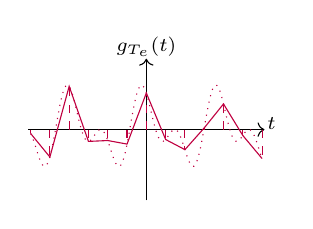
\begin{tikzpicture}
\begin{scope}[scale=0.3]
	\draw[->] (-5,0)-- (5,0);
%\draw (-0.3,-0.3) node {0};
\draw[->] (0,-3)-- (0,3);
\draw (5.3,0.25) node {\scriptsize $t$};
\draw (0,3.5) node {\scriptsize $g_{T_{e}}(t)$};
%\draw (4.5,-0.3) node {1};

\draw[domain=-4.9:4.9,color=purple,samples=13] plot (\x,{2*(0.55*cos(2*\x r)+ 0.45*cos(2*2*(\x+3.14/12) r))}); %0.6125 between each 

\draw[dotted,domain=-4.9:4.9,color=purple,samples=160] plot (\x,{2*(0.55*cos(2*\x r)+ 0.45*cos(2*2*(\x+3.14/12) r))});

\draw[dashed,domain=-4.9:4.9,color=purple,samples=13] plot[ycomb] (\x,{2*(0.55*cos(2*\x r)+ 0.45*cos(2*2*(\x+3.14/12) r))});

\end{scope}
\end{tikzpicture}
\end{center}

\begin{center}
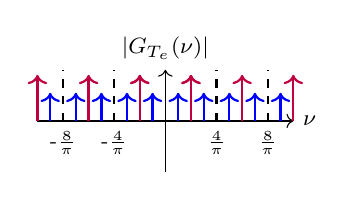
\begin{tikzpicture}
\begin{scope}[scale=0.65]
\draw[->] (-2.5,0)--(2.5,0) node[right]{\footnotesize{$\nu$}};
\draw[->] (0,-1)--(0,1) node[above]{\footnotesize{$|G_{T_e}(\nu)|$}};
\draw[->,blue,thick] (-1/4,0) --(-1/4,0.55) ;
\draw[->,blue,thick] (1/4,0) --(1/4,0.55) ;
\draw[->,purple,thick] (-2/4,0) --(-2/4,0.9) ;
\draw[->,purple,thick] (2/4,0) --(2/4,0.9) ;%\draw[dashed] (-2,0) ellipse (0.25 and 0.5) ;
%\draw[dashed] (2,0) ellipse (0.25 and 0.5) ;
\begin{scope}[xshift=1cm]
\draw[->,blue,thick] (-1/4,0) --(-1/4,0.55) ;
\draw[->,blue,thick] (1/4,0) --(1/4,0.55) ;
\draw[->,purple,thick] (-2/4,0) --(-2/4,0.9) ;
\draw[->,purple,thick] (2/4,0) --(2/4,0.9) ;
\draw[dashed,black,thick] (0,0) node[below]{\scriptsize{$\frac{4}{\pi}$}} --(0,1) ;
\end{scope}

\begin{scope}[xshift=-1cm]
\draw[->,blue,thick] (-1/4,0) --(-1/4,0.55) ;
\draw[->,blue,thick] (1/4,0) --(1/4,0.55) ;
\draw[->,purple,thick] (-2/4,0) --(-2/4,0.9) ;
\draw[->,purple,thick] (2/4,0) --(2/4,0.9) ;
\draw[dashed,black,thick] (0,0) node[below]{\scriptsize{-$\frac{4}{\pi}$}} --(0,1) ;
\end{scope}

\begin{scope}[xshift=2cm]
\draw[->,blue,thick] (-1/4,0) --(-1/4,0.55) ;
\draw[->,blue,thick] (1/4,0) --(1/4,0.55) ;
%\draw[->,purple,thick] (-2/4,0) --(-2/4,0.9) ;
\draw[->,purple,thick] (2/4,0) --(2/4,0.9) ;
\draw[dashed,black,thick] (0,0) node[below]{\scriptsize{$\frac{8}{\pi}$}} --(0,1) ;
\end{scope}

\begin{scope}[xshift=-2cm]
\draw[->,blue,thick] (-1/4,0) --(-1/4,0.55) ;
\draw[->,blue,thick] (1/4,0) --(1/4,0.55) ;
\draw[->,purple,thick] (-2/4,0) --(-2/4,0.9) ;
%\draw[->,purple,thick] (2/4,0) --(2/4,0.55) ;
\draw[dashed,black,thick] (0,0) node[below]{\scriptsize{-$\frac{8}{\pi}$}} --(0,1) ;
\end{scope}
\end{scope}
\end{tikzpicture}
\footnotesize{Shannon pas respecté}
\end{center}

\column{40mm}
\begin{center}
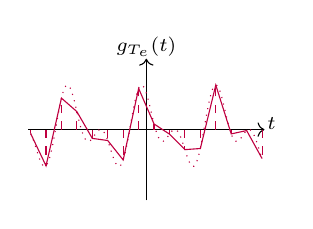
\begin{tikzpicture}
\begin{scope}[scale=0.3]
	\draw[->] (-5,0)-- (5,0);
%\draw (-0.3,-0.3) node {0};
\draw[->] (0,-3)-- (0,3);
\draw (5.3,0.25) node {\scriptsize $t$};
\draw (0,3.5) node {\scriptsize $g_{T_{e}}(t)$};
%\draw (4.5,-0.3) node {1};

\draw[domain=-4.9:4.9,color=purple,samples=16] plot (\x,{2*(0.55*cos(2*\x r)+ 0.45*cos(2*2*(\x+3.14/12) r))}); %0.6125 between each 

\draw[dotted,domain=-4.9:4.9,color=purple,samples=160] plot (\x,{2*(0.55*cos(2*\x r)+ 0.45*cos(2*2*(\x+3.14/12) r))});

\draw[dashed,domain=-4.9:4.9,color=purple,samples=16] plot[ycomb] (\x,{2*(0.55*cos(2*\x r)+ 0.45*cos(2*2*(\x+3.14/12) r))});

\end{scope}
\end{tikzpicture}
\end{center}

\begin{center}
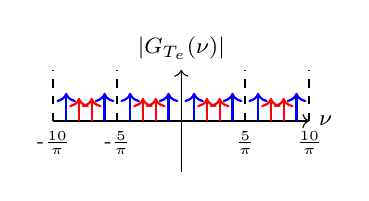
\begin{tikzpicture}
\begin{scope}[scale=0.65]
\draw[->] (-2.5,0)--(2.5,0) node[right]{\footnotesize{$\nu$}};
\draw[->] (0,-1)--(0,1) node[above]{\footnotesize{$|G_{T_e}(\nu)|$}};
\draw[->,blue,thick] (-1/4,0) --(-1/4,0.55) ;
\draw[->,blue,thick] (1/4,0) --(1/4,0.55) ;
\draw[->,red,thick] (-2/4,0) --(-2/4,0.45) ;
\draw[->,red,thick] (2/4,0) --(2/4,0.45) ;%\draw[dashed] (-2,0) ellipse (0.25 and 0.5) ;
%\draw[dashed] (2,0) ellipse (0.25 and 0.5) ;
\begin{scope}[xshift=1.25cm]
\draw[->,blue,thick] (-1/4,0) --(-1/4,0.55) ;
\draw[->,blue,thick] (1/4,0) --(1/4,0.55) ;
\draw[->,red,thick] (-2/4,0) --(-2/4,0.45) ;
\draw[->,red,thick] (2/4,0) --(2/4,0.45) ;
\draw[dashed,black,thick] (0,0) node[below]{\scriptsize{$\frac{5}{\pi}$}} --(0,1) ;
\end{scope}

\begin{scope}[xshift=-1.25cm]
\draw[->,blue,thick] (-1/4,0) --(-1/4,0.55) ;
\draw[->,blue,thick] (1/4,0) --(1/4,0.55) ;
\draw[->,red,thick] (-2/4,0) --(-2/4,0.45) ;
\draw[->,red,thick] (2/4,0) --(2/4,0.45) ;
\draw[dashed,black,thick] (0,0) node[below]{\scriptsize{-$\frac{5}{\pi}$}} --(0,1) ;
\end{scope}

\begin{scope}[xshift=2.5cm]
\draw[->,blue,thick] (-1/4,0) --(-1/4,0.55) ;
%\draw[->,blue,thick] (1/4,0) --(1/4,0.55) ;
\draw[->,red,thick] (-2/4,0) --(-2/4,0.45) ;
%\draw[->,purple,thick] (2/4,0) --(2/4,0.45) ;
\draw[dashed,black,thick] (0,0) node[below]{\scriptsize{$\frac{10}{\pi}$}} --(0,1) ;
\end{scope}

\begin{scope}[xshift=-2.5cm]
%\draw[->,blue,thick] (-1/4,0) --(-1/4,0.55) ;
\draw[->,blue,thick] (1/4,0) --(1/4,0.55) ;
%\draw[->,red,thick] (-2/4,0) --(-2/4,0.45) ;
\draw[->,red,thick] (2/4,0) --(2/4,0.45) ;
\draw[dashed,black,thick] (0,0) node[below]{\scriptsize{-$\frac{10}{\pi}$}} --(0,1) ;
\end{scope}
\end{scope}
\end{tikzpicture}
\footnotesize{Shannon respecté}
\end{center}


\end{columns}
\only<2>
{
\begin{block}{}
Lorsque Shannon n'est pas respecté il y a \textbf{repliement spectral}
\end{block}
}
\end{frame}

\begin{frame}
\frametitle{Impact de l'échantillonnage sur le spectre}

Donc, soit un signal $s(t)$, de spectre $S(\nu)$, alors,  \[ TF(s_{T_e}(t)) =  \frac{1}{T_e}\sum_{n = -\infty}^{\infty} S(\nu - \frac{n}{T_e})) \]   

\begin{columns}
\column{60mm}
\begin{center}
\begin{tikzpicture}
\draw[->] (-2.5,0)--(2.5,0) node[right]{\footnotesize{$\nu$}};
\draw[->] (0,-1)--(0,1) node[above]{\footnotesize{$|S(\nu)|$}};
\draw[blue]  (-0.5,0)--(-0.25,0.5)--(0.25,0.5)--(0.5,0);
\end{tikzpicture}
\end{center}
\column{60mm}
\begin{center}
\begin{tikzpicture}
\draw[->] (-2.5,0)--(2.5,0) node[right]{\footnotesize{$\nu$}};
\draw[->] (0,-1)--(0,1) node[above]{\footnotesize{$|S_{T_e}(\nu)|$}};
\draw[blue]  (-0.5,0)--(-0.25,0.5)--(0.25,0.5)--(0.5,0);
\draw[blue]  (-0.5+2,0)--(-0.25+2,0.5)--(0.25+2,0.5)--(0.5+2,0);
\draw[blue]  (-0.5-2,0)--(-0.25-2,0.5)--(0.25-2,0.5)--(0.5-2,0);
\draw (-2,-0.5)node{$\nu_e$};
\draw (2,-0.5)node{$\nu_e$};
\end{tikzpicture}
\end{center}

\end{columns}

\begin{block}{}
Le spectre du signal échantillonnée est constitué de répétitions du spectre du signal original répété tous les $\nu_e = \frac{1}{T_e}$
\end{block}
\end{frame}


\begin{frame}
\frametitle{Impact de l'échantillonnage sur le spectre}

Donc, soit un signal $s(t)$, de spectre $S(\nu)$, alors,  \[ TF(s_{T_e}(t)) =  \frac{1}{T_e}\sum_{n = -\infty}^{\infty} S(\nu - \frac{n}{T_e})) \]   

\begin{columns}
\column{60mm}
\begin{center}
\begin{tikzpicture}
\draw[->] (-2.5,0)--(2.5,0) node[right]{\footnotesize{$\nu$}};
\draw[->] (0,-1)--(0,1) node[above]{\footnotesize{$|S(\nu)|$}};
\draw[blue]  (-0.5,0)--(-0.25,0.5)--(0.25,0.5)--(0.5,0);
\end{tikzpicture}
\end{center}
\column{60mm}
\begin{center}
\begin{tikzpicture}
\draw[->] (-2.5,0)--(2.5,0) node[right]{\footnotesize{$\nu$}};
\draw[->] (0,-1)--(0,1) node[above]{\footnotesize{$|S_{T_e}(\nu)|$}};
\draw[blue]  (-0.5,0)--(-0.25,0.5)--(0.25,0.5)--(0.5,0);
\draw[blue]  (-0.5+0.75,0)--(-0.25+0.75,0.5)--(0.25+0.75,0.5)--(0.5+0.75,0);
\draw[blue]  (-0.5-0.75,0)--(-0.25-0.75,0.5)--(0.25-0.75,0.5)--(0.5-0.75,0);
\draw (-2,-0.5)node{$\nu_e$};
\draw (2,-0.5)node{$\nu_e$};
\end{tikzpicture}
\end{center}

\end{columns}

\begin{block}{}
\textbf{Repliement spectral} :  Superposition des fréquencees dans les répliques dûe à une fréquence d'échantillonnage $\nu_e$ trop basse
\end{block}


\end{frame}


\begin{frame}
\frametitle{Signaux discrets : aspects matériels}
\small{Pour passer d'un signal analogique à un signal "temps discret/amplitude discrète", on utilise des \textbf{convertisseurs analogique-numérique}}\\
\vspace{0.5cm}

\begin{columns}
\column{40mm}
\begin{circuitikz} \draw
(0,0) node[op amp] (opamp) {}
 (opamp.+) node[left] {$v_+$}
 (opamp.-) node[left] {$v_-$}
 (opamp.out) node[right] {$v_o$};
 \end{circuitikz}\\
 \footnotesize{Symbole d'un amplificateur opérationnel}
 \column{80mm}
 Ces circuits sont généralements constitués :
 \vspace{0.2cm}
 \begin{itemize}
 \item Ampli-ops utilisés comme comparateurs
 \vspace{0.3cm}
 \item Horloge
 \vspace{0.3cm} 
 \item Circuit de charge/décharge
 \end{itemize}
 \end{columns}
\end{frame}

\begin{frame}
\frametitle{Signaux discrets : aspects matériels}
\begin{columns}
\column{40mm}
\begin{center}
 \begin{circuitikz} \draw
 (0,0) to[short,o-] ++(0.3,0)
 to[adc,>] ++(2,0)
to[short,-o] ++(0.3,0);
 \end{circuitikz}\\
 \footnotesize{schéma d'un convertisseur analogique-numérique}
\end{center}
 \column{80mm}
\small{\underline{Fonctionnement }:
 \vspace{0.2cm}
 \begin{enumerate}
 \item La tension en entrée est maintenue pendant un cycle d'horloge
 \vspace{0.3cm}
 \item le convertisseur effectue les opérations de conversion 
 \vspace{0.3cm} 
 \item Le convertisseur délivre sur ses sorties (dépend du nombre de bits) le code correspondant à la valeur binaire (ex : 0011) 
 \end{enumerate}
 }
 \end{columns}
\begin{block}{}
Comment maintenir la tension pendant un cycle complet ?
\end{block}
\end{frame}

\begin{frame}
\frametitle{Signaux discrets : aspects matériels}
\underline{\'Echantillonneur-bloqueur:}\\
\begin{center}
\includegraphics[scale=0.15]{sample_hold.png}\\
\footnotesize{Schéma du circuit. $AI$ = entrée analogique, $AO$ = sortie analogique, $C$ = commande}
\end{center}
\vspace{0.2cm}
\small{
\begin{itemize}
\item Lorsqu'on ouvre $C$, la valeur de $AI$ se maintient sur $AO$
\item Les composants triangulaires sont aussi des ampli-op
\item Cette configuration évite également les chutes de tensions en sortie 
\end{itemize}
}
%\begin{circuitikz} \draw
%(0,0) node[op amp] (opamp) {}
% (opamp.+) node[left] {$v_+$}
% (opamp.-) node[left] {$v_-$}
% (opamp.out) node[right] {$v_o$};
% \end{circuitikz}
\end{frame}


\subsection{Transformée en $z$}

\begin{frame}
\frametitle{Transformée en $z$: Définition}
Transformées de Fourier et de Laplace $\rightarrow$ Analyse systèmes à fonctions continues\\

\vspace{0.3 cm}

\only<2->{
Transformée en Z $\rightarrow$ analyse systèmes à fonctions discrètes (numériques)\\
}


\only<3->{
\vspace{0.3 cm}
Soit $s[n]$ un signal discret, \\
\[TZ\{ f \}(z) = \sum_{n = -\infty}^{\infty} f[n] z^{-n} \]
}
 \vspace{0.3 cm}

\only<4->{
Tout comme la transformée de Laplace il existe aussi une variante monolatérale:

\[TZ\{ f \}(z) = \sum_{n = 0}^{\infty} f[n] z^{-n} \]
}

\end{frame} 

\begin{frame}
\frametitle{Transformée en $z$: Définition}
\[TZ\{ f \}(z) = \sum_{n = 0}^{\infty} f[n] z^{-n} \]

\vspace{0.3 cm} 
\only<2->{
fonction de $t$ \textbf{échantillonnée} $\rightarrow$ fonction de $z$ \textbf{continue}\\
}
\vspace{0.3 cm} 
\only<3->{
La transformée en $z$ est une fonction \textbf{complexe}
}

\end{frame} 


\begin{frame}
\frametitle{Propriétés de la transformée en $z$}
Par construction, même propriétés que Laplace et Fourier\\
\vspace{0.4cm}

\begin{itemize}
\item<2-> Linéarité \only<3->{: \[TZ(a x_1[n] + b x_2[n]) = a\cdot TZ (x_1[n]) + b\cdot TZ(x_2[n]) \]}
\vspace{0.3cm}
\item<4-> Convolution \only<5->{: \[TZ(x_1[n] \star x_2[n]) = TZ(x_1) TZ(x_2)\]}
\vspace{0.3cm}
\item<6-> Décalage temporel \only<6->{: \[ TZ\{x[n-k]\} = X(z)\cdot z^{-k} \]}
\end{itemize}

\end{frame}

\begin{frame} 
\frametitle{Quelques transformées en $z$ usuelles}
Soit $\delta [n]$ l'impulsion de Kronecker,
\vspace{0.3 cm}
\[TZ\{ \delta[n] \} = \sum_{n = 0}^{\infty} \delta[n] z^{-n}\]

\vspace{0.3 cm}
\only<2->{
\[\sum_{n = 0}^{\infty} \delta[n] \; z^{-n} = z^0 =  1 \]
}

\vspace{0.3 cm}
\only<3->{

\[ \boxed{TZ\{ \delta[n] \} =  1} \]

}
\vspace{0.4cm}
\only<4->{ Résultat similaire en Laplace et en Fourier}

\end{frame}

\begin{frame} 
\frametitle{Quelques transformées en $z$ usuelles}

Soit $u [n]$ l'échelon échantillonné,

\[TZ\{ u[n] \} = \sum_{n = 0}^{\infty} u[n] \; z^{-n}  \]

\vspace{0.3cm}
\only<2->{
\[\boxed{TZ\{ u[n] \} = \sum_{n = 0}^{\infty} z^{-n}  = \frac{1}{1-z^{-1}}} \]

\vspace{0.3cm}
Vrai si $|z|>1$ (série géométrique)

}
\end{frame} 

\begin{frame} 
\frametitle{Quelques transformées en $z$ usuelles}

Soit $n\cdot u [n]$ la rampe échantillonnée,

\[TZ\{ n\cdot u[n] \} = \sum_{n = 0}^{\infty} n \cdot u[n] \; z^{-n} \]

\vspace{0.3cm}

\only<2->{
\[\boxed{TZ\{ n\cdot u[n] \}  = \frac{z^{-1}}{(1-z^{-1})^2}} \]
}

\end{frame}

%\begin{frame} 
%\frametitle{Quelques transformées en $z$ usuelles}
%
%Soit $\sin(\omega_0 \cdot n )\cdot u [n]$ le sinus échantillonné,
%
%\vspace{0.3cm}
%
%\only<2->{
%\[\boxed{TZ\{ \sin(\omega_0 \cdot n )\cdot u [n] \}  = \frac{z^{-1} \sin(\omega_0)}{1-2z^{-1} \cos(\omega_0) +z^{-2}}} \]
%}
%\end{frame}

\begin{frame}
\frametitle{Quelques transformées en $z$ usuelles}

\begin{enumerate}
\item $\delta[n] \rightarrow  1$ 
\vspace{0.3cm}
\item $u[n] \rightarrow \frac{\displaystyle 1}{ \displaystyle 1-z^{-1}}$
\vspace{0.3cm}
\item $n \cdot u[n] \rightarrow \frac{\displaystyle z^{-1}}{\displaystyle (1-z^{-1})^2} $
\vspace{0.3cm}
%\item $\sin(\omega_0 n) \cdot u(n) \rightarrow  \frac{\displaystyle z^{-1} \sin(\omega_0)}{\displaystyle 1-2z^{-1} \cos(\omega_0) +z^{-2}} $
\end{enumerate} 
\vspace{0.5cm}

Fonctions rencontrées fréquemment en traitement du signal numérique.

\end{frame}

\begin{frame}
\frametitle{Transformée en $z$ Lien avec Fourier et Laplace}

Remarque : La transformée en $z$ ne fait pas intervenir la période d'échantillonnage $T_e$...\\
\begin{columns}
\column{60mm}
\begin{center}
\begin{tikzpicture}
\begin{scope}[scale=0.4]
	\draw[->] (-5,0)-- (5,0);
%\draw (-0.3,-0.3) node {0};
\draw[->] (0,-3)-- (0,3);
\draw (5.3,0.25) node {\scriptsize $n$};
\draw (0,3.5) node {\scriptsize $u[n]$};

\draw[domain=-4.9:4.9,color=blue,samples=16] plot[ycomb] (\x,{2*(0.55*cos(2*\x r)+ 0.45*cos(2*2*(\x+3.14/12) r))});

\end{scope}
\end{tikzpicture}
\end{center}
\column{60mm}
\begin{itemize}
\item Même résultat pour n'importe quel $T_e$
\vspace{0.3cm}
\item La TZ analyse l'enchaînement des échantillons
\end{itemize}

\end{columns}
\end{frame}

\begin{frame}
\frametitle{Transformée en $z$ Lien avec Fourier et Laplace}

Remarque : La transformée en $z$ ne fait pas intervenir la période d'échantillonnage $T_e$...\\

\vspace{1cm}
\only<2->{
Si on souhaite "retrouver" cette variable, il faut repasser de $z$ à Laplace ou Fourier...\\
}

\vspace{1cm}
\only<3->{
\begin{columns}
\column{60mm}
Laplace : 

\[ \boxed{z = e^{sT_e}} \] 

\column{60mm}
Fourier :
\[\boxed{ z = e^{j\omega T_e} = e^{j 2 \pi \nu T_e}} \]
\end{columns}
}

\end{frame}

\subsection{Transformée de Fourier Discrète}
\subsubsection{Définition}
\begin{frame}
\frametitle{Transformée de Fourier...}
On résume... Soit $x[n]$ un signal discret,\\
\vspace{0.3cm}
\only<2->{
\[TZ\{ x[n] \} \rightarrow TF\{x[n]\} =  \sum_{{\color{blue!50!cyan}n = -\infty}}^{{\color{blue!50!cyan}\infty}} x[n] e^{-j 2 \pi n {\color{blue!40!green} \nu }T_e}\] \\

\vspace{0.3cm}
{\color{blue!50!cyan}Somme infinie}... Et {\color{blue!40!green}variable fréquentielle continue}\\
\vspace{0.3cm}
}
\only<3->{
\begin{block}{}
Comment calculer une transformée de Fourier avec un ordinateur ?
\end{block}
}

\end{frame} 

\begin{frame}
\frametitle{Transformée de Fourier...Discrète}
Sur ordinateur ou support numérique, il faut :\\ 
\vspace{0.3cm}
\begin{enumerate}
\item<2-> Sommer sur un nombre fini de termes
\vspace{0.3cm}
\item<3-> Calculer le spectre pour un nombre fini de valeurs en fréquence 
\end{enumerate}

\vspace{0.3cm}
\only<4->{
donc ,
}
\vspace{0.3cm}

\only<5->{ \[ TF\{ x \}(\nu) = \sum_{{\color{blue!50!cyan}n = 0}}^{{\color{blue!50!cyan}\infty}} x[n] \; e^{-j 2 \pi n \nu T_e} \rightarrow  \sum_{{\color{blue!50!cyan}n = 0}}^{{\color{blue!50!cyan}N-1}} x[n] \; e^{-j 2 \pi n \nu T_e} \]}\vspace{0.2cm}
\only<6->{ \[ \sum_{n = 0}^{N-1} x[n] \; e^{-j 2 \pi n {\color{blue!40!green}\nu} T_e} \rightarrow TF(x)[m] = \sum_{n = 0}^{N-1} x[n] \; e^{-j 2 \pi n {\color{blue!40!green} m \frac{\nu_e}{N}} T_e }  \]}
\end{frame}

\begin{frame}
\frametitle{Transformée de Fourier...Discrète}

 \[ TF\{ x \}(\nu) = \sum_{{\color{blue!50!cyan}n = 0}}^{{\color{blue!50!cyan}\infty}} x[n] \; e^{-j 2 \pi n \nu T_e} \rightarrow  \sum_{{\color{blue!50!cyan}n = 0}}^{{\color{blue!50!cyan}N-1}} x[n] \; e^{-j 2 \pi n \nu T_e} \]
\[ \sum_{n = 0}^{N-1} x[n] \; e^{-j 2 \pi n {\color{blue!40!green}\nu} T_e} \rightarrow TF(x)[m] = \sum_{n = 0}^{N-1} x[n] \; e^{-j 2 \pi n {\color{blue!40!green} m \frac{\nu_e}{N}} T_e }  \]
On note que $\nu_e T_e = 1$

\only<2-> {\[\sum_{n = 0}^{N-1} x[n] \; e^{-j 2 \pi n m \frac{\nu_e}{N} T_e } = \sum_{n = 0}^{N-1} x[n] \; e^{-j 2 \pi n \frac{m}{N} }\]}

\end{frame}



\begin{frame}
\frametitle{Transformée de Fourier Discrète (TFD)}
En résumé,\\
\vspace{0.3cm} 
\[ TFD\{ x \}[m] = \frac{1}{N} \sum_{n = 0}^{N-1} x[n] \; e^{-j 2 \pi n \frac{m}{N}}  \] 
\begin{itemize}
\item $m$ : indice dans l'espace des fréquences
\item $n$ : variable de sommation
\item $N$ : nombre de termes sommation/espace des fréquences
\end{itemize}
\vspace{0.3cm}
\begin{itemize}
\item<2-> C'est cette fonction que MATLAB ou Python calcule
\vspace{0.3cm}
\item<3-> Formulée ainsi, la TFD comme la transformée en $z$, ne fait pas intervenir $T_e$  
\end{itemize}

\end{frame}

\subsubsection{Lien avec la TFD}
\begin{frame} 
\frametitle{Lien entre TF et TFD}

\[\text{Transformée de Fourier: }X(\nu) = \sum_{n = -\infty}^{\infty} x[n] \; e^{-j 2 \pi n \nu T_e}\] 
\vspace{0.2cm}
\begin{itemize}
\item<2-> Somme infinie sur signal discret
\vspace{0.2cm}
\item<3-> Spectre en fréquence continu (infinité de points)
\end{itemize}
\vspace{1cm}
\[\text{Transformée de Fourier Discrète} :X_D(m) = \sum_{n = 0}^{N-1} x[n] \; e^{-j 2 \pi n \frac{m}{N} }\]
\vspace{0.2cm}
\begin{itemize}
\item<2-> Somme finie ($N$) sur signal discret 
\vspace{0.2cm}
\item<3-> Spectre en fréquence fini et échantillonné sur $N$ points.
\end{itemize}

\end{frame}

%\begin{frame} 
%\frametitle{TZ, TF et TFD: exemple}
%
%Soit $u [n]$ l'échelon échantillonné,\\
%
%\[TZ\{ u[n] \} = \sum_{n = 0}^{\infty} u[n] \; z^{-n} = \frac{1}{1-z^{-1}}  \]
%
%\only<2->{
%\[TF\{ u[n] \}(\nu) = U(\nu) =   \frac{1}{1-e^{-j 2 \pi \nu T_e}}  \]
%}
%
%\only<3->{
%\vspace{0.3cm}
%On calcule le module de cette fonction pour avoir le spectre en amplitude
%}
%
%\only<4->{
% \[ |U(\nu)| =   \frac{1}{2 \sin(\pi \nu T_e)}  \]
%
%}
%
%\end{frame} 
%
%\begin{frame} 
%\frametitle{TZ, TF et TFD: exemple}
%Analysons la fonction
% \[ |U(\nu)| =   \frac{1}{|2 \sin(\pi \nu T_e)|}  \]
%\only<2->{
%fonction périodique de période $\nu_e$
%}
%\only<3->{
%\begin{center}
%\begin{tikzpicture}
%\begin{scope}[scale=0.8]
%	\draw[->] (-2,0)-- (2,0);
%%\draw (-0.3,-0.3) node {0};
%\draw[->] (0,0)-- (0,3);
%\draw (2.3,0.25) node {\scriptsize $\nu$};
%\draw (0,3.5) node {\scriptsize $U(\nu)$};
%
%\draw[domain=-1.95:-1.05,color=blue,samples=32] plot (\x,{1/(abs(2*sin(3.14*\x r))))});
%\draw[domain=-0.95:-0.05,color=blue,samples=32] plot (\x,{1/(abs(2*sin(3.14*\x r))))});
%\draw[domain=0.05:0.95,color=blue,samples=32] plot (\x,{1/(abs(2*sin(3.14*\x r))))});
%\draw[domain=1.05:1.95,color=blue,samples=32] plot (\x,{1/(abs(2*sin(3.14*\x r))))});
%
%\draw[dashed] (1,0)--(1,3);
%\draw[dashed] (-1,0)--(-1,3);
%\draw[dashed] (2,0)--(2,3);
%\draw[dashed] (-2,0)--(-2,3);
%
%\draw (1,-0.3) node{\footnotesize{$\nu_e$}};
%\end{scope}
%\end{tikzpicture}
%\end{center}
%}
%\end{frame} 
%
%\begin{frame}
%\frametitle{TFD: Exemple}
%\begin{columns}
%\column{50mm}
%\begin{center}
%\begin{tikzpicture}
%\begin{scope}[scale=0.3]
%	\draw[->] (-5,0)-- (5,0);
%%\draw (-0.3,-0.3) node {0};
%\draw[->] (0,-3)-- (0,3);
%\draw (5.3,0.25) node {\scriptsize $t$};
%\draw (0,3.5) node {\scriptsize $g_{T_{e}}(t)$};
%%\draw (4.5,-0.3) node {1};
%
%\draw[domain=-4.9:4.9,color=purple,samples=16] plot (\x,{2*(0.55*cos(2*\x r)+ 0.45*cos(2*2*(\x+3.14/12) r))}); %0.6125 between each 
%
%\draw[dotted,domain=-4.9:4.9,color=purple,samples=160] plot (\x,{2*(0.55*cos(2*\x r)+ 0.45*cos(2*2*(\x+3.14/12) r))});
%
%\draw[dashed,domain=-4.9:4.9,color=purple,samples=16] plot[ycomb] (\x,{2*(0.55*cos(2*\x r)+ 0.45*cos(2*2*(\x+3.14/12) r))});
%
%\end{scope}
%\end{tikzpicture}
%\end{center}
%
%\begin{center}
%\begin{tikzpicture}
%\begin{scope}[scale=0.65]
%\draw[->] (-2.5,0)--(2.5,0) node[right]{\footnotesize{$\nu$}};
%\draw[->] (0,-1)--(0,1) node[above]{\footnotesize{$|G_{T_e}(\nu)|$}};
%\draw[->,blue,thick] (-1/4,0) --(-1/4,0.55) ;
%\draw[->,blue,thick] (1/4,0) --(1/4,0.55) ;
%\draw[->,red,thick] (-2/4,0) --(-2/4,0.45) ;
%\draw[->,red,thick] (2/4,0) --(2/4,0.45) ;%\draw[dashed] (-2,0) ellipse (0.25 and 0.5) ;
%%\draw[dashed] (2,0) ellipse (0.25 and 0.5) ;
%\begin{scope}[xshift=1.25cm]
%\draw[->,blue,thick] (-1/4,0) --(-1/4,0.55) ;
%\draw[->,blue,thick] (1/4,0) --(1/4,0.55) ;
%\draw[->,red,thick] (-2/4,0) --(-2/4,0.45) ;
%\draw[->,red,thick] (2/4,0) --(2/4,0.45) ;
%\draw[dashed,black,thick] (0,0) node[below]{\scriptsize{$\frac{5}{\pi}$}} --(0,1) ;
%\end{scope}
%
%\begin{scope}[xshift=-1.25cm]
%\draw[->,blue,thick] (-1/4,0) --(-1/4,0.55) ;
%\draw[->,blue,thick] (1/4,0) --(1/4,0.55) ;
%\draw[->,red,thick] (-2/4,0) --(-2/4,0.45) ;
%\draw[->,red,thick] (2/4,0) --(2/4,0.45) ;
%\draw[dashed,black,thick] (0,0) node[below]{\scriptsize{-$\frac{5}{\pi}$}} --(0,1) ;
%\end{scope}
%
%\begin{scope}[xshift=2.5cm]
%\draw[->,blue,thick] (-1/4,0) --(-1/4,0.55) ;
%%\draw[->,blue,thick] (1/4,0) --(1/4,0.55) ;
%\draw[->,red,thick] (-2/4,0) --(-2/4,0.45) ;
%%\draw[->,purple,thick] (2/4,0) --(2/4,0.45) ;
%\draw[dashed,black,thick] (0,0) node[below]{\scriptsize{$\frac{10}{\pi}$}} --(0,1) ;
%\end{scope}
%
%\begin{scope}[xshift=-2.5cm]
%%\draw[->,blue,thick] (-1/4,0) --(-1/4,0.55) ;
%\draw[->,blue,thick] (1/4,0) --(1/4,0.55) ;
%%\draw[->,red,thick] (-2/4,0) --(-2/4,0.45) ;
%\draw[->,red,thick] (2/4,0) --(2/4,0.45) ;
%\draw[dashed,black,thick] (0,0) node[below]{\scriptsize{-$\frac{10}{\pi}$}} --(0,1) ;
%\end{scope}
%\end{scope}
%\end{tikzpicture}
%\end{center}
%\column{70mm}
%\[g(t) = 0.55{\color{blue}\cos(2 t)} + 0.45 {\color{red}\cos(4 t + \frac{\pi}{3})} \]
%
%\[ TF(g_{T_e}(t)) =  \frac{1}{T_e}\sum_{n = -\infty}^{\infty} G(\nu - \frac{n}{T_e})) \] 
%
%\vspace{0.5cm}
%Quelle est la TFD du signal ?
%\end{columns}
%\end{frame}

%

\subsubsection{Zero padding}
\begin{frame}
\frametitle{TFD et zero padding}
Peu de points dans le signal = peu de points dans le spectre...\\

\vspace{0.1cm}
\[
\begin{bmatrix} x[1] \\ x[2] \\ \vdots \\ x[N] \end{bmatrix} \; -TFD \rightarrow  
\begin{bmatrix} X[1] \\ X[2] \\ \vdots \\ X[N] \end{bmatrix}
\]
\vspace{0.1cm}
\only<2->{Solution:  Zero padding - on ajoute M zéros derrière le vecteur signal
\[
\begin{bmatrix} x[1] \\ x[2] \\ \vdots \\ x[N] \\ 0 \\ \vdots \\ 0 \end{bmatrix} \; -TFD \rightarrow  
\begin{bmatrix} X[1] \\ X[2] \\ \vdots \\  \vdots \\  \vdots \\ X[N+M] \end{bmatrix}
\]}

\end{frame} 

\begin{frame}
\frametitle{TFD et zero padding}

\[
\begin{bmatrix} x[1] \\ x[2] \\ \vdots \\ x[N] \\ 0 \\ \vdots \\ 0 \end{bmatrix} \; -TFD \rightarrow  
\begin{bmatrix} X[1] \\ X[2] \\ \vdots \\  \vdots \\  \vdots \\ X[N+M] \end{bmatrix}
\]
\vspace{0.5cm}

"Interpole" le spectre de façon à avoir plus de points avec le \textbf{même signal}

\only<2->{
\vspace{0.5cm}
\textbf{Attention:} Le zéro padding ne crée pas d'information
}
\end{frame}

\begin{frame}
\frametitle{TFD et zero padding :Exemple}

\begin{columns}
\column{60mm}
\begin{center}
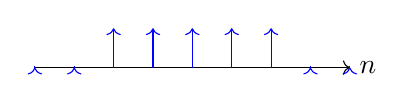
\begin{tikzpicture}
\begin{scope}[scale =0.5]
\draw[->](-4,0)--(4,0) node[right]{$n$};
%\draw(0,-2)--(0,2) node[right]{$x[n]$};

\draw[->,blue](-4,0)--(-4,0);
\draw[->,blue](-3,0)--(-3,0);
\draw[->,blue](-2,0)--(-2,1);
\draw[->,blue](-1,0)--(-1,1);
\draw[->,blue](0,0)--(0,1);
\draw[->,blue](1,0)--(1,1);
\draw[->,blue](2,0)--(2,1);
\draw[->,blue](3,0)--(3,0);
\draw[->,blue](4,0)--(4,0);
\end{scope}
\end{tikzpicture}\\
\vspace{0.4cm}
\only<2->{On rajoute 91 zéros derrière les 9 échantillons pour avoir 100 points dans le spectre}
\end{center}

\column{60mm}
\begin{center}
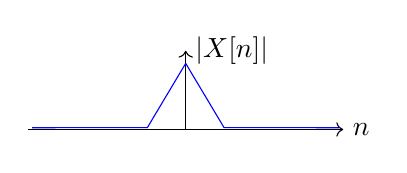
\begin{tikzpicture}
\begin{scope}[scale =0.5]
\draw[->](-4,0)--(4,0) node[right]{$n$};
\draw[->](0,0)--(0,2) node[right]{$|X[n]|$};

\draw[ domain=-3.9:3.9,color=blue,samples=9] plot  (\x,{abs(100*( sin(3.14*\x r  )/(3.14*\x r)))});
\end{scope}
\end{tikzpicture}\\
\vspace{0.9cm}
\only<2->{
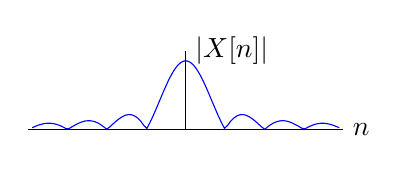
\begin{tikzpicture}
\begin{scope}[scale =0.5]
\draw(-4,0)--(4,0) node[right]{$n$};
\draw(0,0)--(0,2) node[right]{$|X[n]|$};

\draw[ domain=-3.9:3.9,color=blue,samples=100] plot  (\x,{abs(100*( sin(3.14*\x r  )/(3.14*\x r)))});
\end{scope}
\end{tikzpicture}
}
\end{center}
\end{columns}
\vspace{0.5cm}
\only<3->{
En rajoutant des zéros, on se "rapproche" de la transformée de Fourier non-discrète
}
\end{frame}

\begin{frame}
\frametitle{TFD: résumé}
\begin{itemize}
\item TFD calculable par ordi : nombre finis de termes 
\vspace{0.3cm}
\item<2-> Approximation de la TF
\vspace{0.3cm}
\item<3-> Utilisation possible du zéro padding pour rajouter des points au spectre.

\end{itemize}
\vspace{1cm}
Dans tous ces développements, on part du principe que l'amplitude est continue mais ce n'est pas exact (codage)
\end{frame}

\subsection{Résumé du chapitre}
\begin{frame}

\frametitle{Résumé du chapitre}
\begin{enumerate}
\item Signaux numériques
\vspace{0.2cm} 
\begin{itemize}
\item<3->  Codage : discrétisation de l'amplitude 
\vspace{0.3cm}
\item<4->  \'Echantillonnage : discrétisation du temps
\vspace{0.3cm}
\begin{itemize} 
\item  Critère de Shannon : $f_e > 2 f_{max}$
\vspace{0.3cm}
\item  Peigne de Dirac et périodisation du spectre $\rightarrow$ \textbf{Repliement spectral}
\end{itemize} 
\end{itemize}
\vspace{0.3cm}
\item<2-> Transformée en $z$ \& Transformée de Fourier discrète
\vspace{0.2cm} 
\begin{itemize}
\item<5->  Définition TZ \& TZ fonctions usuelles 
\vspace{0.3cm} 
\item<6->  Lien avec Fourier : $z = e^{j \pi f T_e}$
\vspace{0.3cm}
\item<7->  Transformée de Fourier discrète et zero-padding
\begin{itemize} 
\item  Limitation du nombre de termes por les supports numériques
\vspace{0.15cm}
\item  Zéro-padding: Ajout de zéros après les échantillons temporels $\rightarrow$ plus de points dans le spectre
\end{itemize} 
\end{itemize}
\end{enumerate}

\end{frame}
\end{document}